\setchapterpreamble[u]{\margintoc}
\chapter{Results}
\labch{HESE12}
The 7.5 years of HESE data (2010-2017) was previously used to measure the composition of astrophysical neutrino flavours \sidecite[6cm]{Juliana_paper} (in particular to search for $\nu_{\tau}$ events) and energy spectrum \sidecite[7cm]{HESE7_sample}. This dataset included 102 events, (of which 60 events were above 60 TeV), that passed the HESE selection criteria, as outlined in Section~\ref{sec:HESE}. Two events were identified as Double Cascades using the particle identifier described in Section~\ref{sec:PID}. 

For this iteration, the analysis has undergone significant changes compared to previous versions while maintaining consistent selection criteria and particle identification methods. The most notable difference lies in the ice model, specifically its influence on the reconstruction of tau decay length, detailed in Section~\ref{sec:icemodel}. The previous iteration of the analysis used the SPICE-3.2 ice model. The SPICE-Bfr have impacts on the overall energy estimates, as the number of photons collected in a given time window have significantly changed in this model of ice depending on the alignment of DOMs with respect to the iceflow axis \sidecite[3.5cm]{BFR_paper}, as was discussed in Section~\ref{sec:icemodel_checks}. Furthermore, the treatment of detector systematics has evolved, utilizing the SnowStorm method (see Section~\ref{sec:snowstorm}) instead of separate Monte Carlo datasets with discrete variations of parameters related to systematic uncertainties used previously. The update also includes using the revised light-yield tables \sidecite[3.5cm]{updated_recotables_tianlu} for the maximum likelihood reconstruction method described in Section~\ref{sec:reco}. Moreover, the high quantum efficiency DeepCore DOMs were included in the analysis as previously their reponses were excluded from \texttt{millipede} reconstruction methods described in Section~\ref{sec:reco}, as they can introduce biases which was not simulated correctly for high energy simulations. This has now been fixed and hence these DOMs were no longer excluded form the reconstructions.

Additionally, various corrections have been applied to Monte Carlo simulations, by modifying event interaction weights to incorporate corrections due to tau polarization and initial state radiation corrections to the Glashow cross-sections (see Sections \ref{sec:tau_polarisation} and \ref{sec:glashow_correction} for details). Lastly, some of the nuisance parameters, affecting atmospheric spectra and detector responses have been introduced (as described in Section~\ref{sec:params}). Lastly, the analysis software is also different (see Section~\ref{sec:sensitivty}). Hence, as a first step, the 7.5 years of HESE data were re-analysed to make direct comparisons with the previous results and to re-evaluate the anlaysis if necessary.

This chapter presents a new flavour measurements made using ~12 years (11.69 to be exact) of HESE data. It begins by discussing the re-anlaysing of 7.5 years of data, followed by results from the 12-year fit, including a discussion of data / Monte Carlo agreement and detailed post-unblinding checks. Finally, the flavour measurement results are presented and interpreted in the last sections.

\section{(Re)Analysing the 7.5 years of HESE Data}
\label{sec:HESE7}
The re-anlaysing of the HESE-7.5 data (\textbf{Re-analysis Default}), revealed that 64 events met the HESE selection criteria, each with a deposited energy exceeding 60 TeV. It included 6 Double Cascade events, which is a significant increase from the previous analysis (\textbf{HESE-7.5}) that identified only two Double Cascade events. The comparison of these reconstructed variables for both iterations is shown in \reftab{reco_values_comparisons_bfr}. 
\begin{table*}[h!]
    \caption[Comparison of Reconstructed quantities of re-analysed HESE-7.5 data by using Spice-Bfr ice model with published HESE-7.5 events]{Comparison of Reconstructed quantities of events classified as Double Cascades for results obtained using \textbf{Re-analysis Default} and \textbf{HESE-7.5} (grey cells). Shown in the table are (from left), MJD (Modified Julian Date), reconstructed length, reconstructed Energy of first ($\mathrm{E}_1$) and second ($\mathrm{E}_2$) cascades, Energy asymmetry ($\mathrm{E}_\mathrm{A}$), Energy Confinement ($\mathrm{E}_\mathrm{C}$) and classified morphology of the event. The two common events, 57134 (\emph{Double Double}) and 56265 (\emph{Big Bird}) have nearly identical reconstructed quantities.}
    \labtab{reco_values_comparisons_bfr}
    \begin{tabular}{c|cc|cc|cc|cc|cc|cc}
        \toprule
         MJD    & \multicolumn{2}{c|}{Length}
                
                        & \multicolumn{2}{c|}{$\mathrm{E}_\mathrm{1}$}
                                & \multicolumn{2}{c|}{$\mathrm{E}_\mathrm{2}$} 
                                    & \multicolumn{2}{c|}{$\mathrm{E}_\mathrm{A}$} 
                                        & \multicolumn{2}{c|}{$\mathrm{E}_\mathrm{C}$}  
                                            & \multicolumn{2}{c}{morphology}                \\
                       
        \midrule
        57835   &   13 m   & \cellcolor{lightgray}66 m    & 19 TeV   &   \cellcolor{lightgray}79 TeV  &   73 TeV  &   \cellcolor{lightgray}3 TeV  &   -0.58  &   \cellcolor{lightgray}0.93 & 1 &  \cellcolor{lightgray}1&Double& \cellcolor{lightgray}Single\\
            % \hline
        57134   &   17 m   & \cellcolor{lightgray}17 m    & 5.7 TeV   &   \cellcolor{lightgray}8.7 TeV  &   92 TeV  &   \cellcolor{lightgray}79 TeV  &   -0.89  &   \cellcolor{lightgray}-0.80 & 0.99 &  \cellcolor{lightgray}0.99&Double& \cellcolor{lightgray}Double\\
            % \hline
        56603   & 13 m   & \cellcolor{lightgray}70 m    & 32 TeV   &   \cellcolor{lightgray}85 TeV  &    48 TeV  &   \cellcolor{lightgray}1 TeV  &   -0.19  &   \cellcolor{lightgray}1 & 1 &  \cellcolor{lightgray}0.99 & Double & \cellcolor{lightgray}Single\\
            % \hline
        55714   &   14 m   & \cellcolor{lightgray}26 m    & 5 TeV   &   \cellcolor{lightgray}58 TeV  &   82 TeV  &   \cellcolor{lightgray}16 TeV  &   -0.88  &   \cellcolor{lightgray}0.55 & 0.99 &  \cellcolor{lightgray}1&Double& \cellcolor{lightgray}Single\\
            % \hline
        55800   &   13 m   & \cellcolor{lightgray}20 m    & 128 TeV   &   \cellcolor{lightgray}133 TeV  &   72 TeV  &   \cellcolor{lightgray}38 TeV  &   0.28  &   \cellcolor{lightgray}0.55 & 1 &  \cellcolor{lightgray}0.99&Double& \cellcolor{lightgray}Single\\
            % \hline
        56265   &  16 m   & \cellcolor{lightgray}16 m    & 1.1 PeV   &   \cellcolor{lightgray}1.2 PeV  &   0.9 PeV  &   \cellcolor{lightgray}0.6 PeV  &   0.09  &   \cellcolor{lightgray}0.29 & 1 &  \cellcolor{lightgray}1&Double& \cellcolor{lightgray}Double\\
            \bottomrule
    \end{tabular}
\end{table*}

\marginnote{\begin{kaobox}
    To avoid any confusion, the following terms will be used to describe which iteration of the analysis is being discussed:\\
    \textbf{HESE-7.5}: It refers to previoys anlaysis, with results described in \cite{Juliana_paper}\\
    \textbf{Re-analysis Legacy}: Re analysed results using SPICE-3.2.1 ice model\\
    \textbf{Re-analysis Default} : Re analysed results using SPICE-Bfr ice model\\
\end{kaobox}}

A key difference in this iteration was the ice model used for reconstruction, as mentioned before. Hence, the data was re-analysed using both SPICE-3.2.1 and SPICE-Bfr to make direct comparisons with the previous results, and to check if the observed surplus of events is due to this new ice model. The re-analysis using SPICE-3.2.1 (\textbf{Re-analysis Legacy}) contained total of 62 HESE events above 60 TeV deposited energy, of which 7 events were classified as Double Cascades, the reconstructed properties and their comparisons with HESE-7.5 is shown in \reftab{reco_values_comparisons_spice}. Notably, 5 of the 7 double cascade events had been classified as single cascades in the previous analysis. The most striking differences here are specifically reconstructed length and the fact that $\mathrm{E}_1$ and $\mathrm{E}_2$ seem to be almost flipped for some events, even though reconstructed directions (zenith and azimuth, not shown in the table) remains almost idnetical. Despite the changes in the total number of classified events, the two common Double Cascade events identified in both iterations (Re-analysis Legacy and HESE-7.5) exhibited nearly identical reconstructed properties.

\begin{table*}[h!]
    \caption[Comparison of Reconstructed quantities of re-analysed HESE-7.5 data by using Spice-Bfr ice model with published HESE-7.5 events]{Comparison of Reconstructed quantities of events classified as Double Cascades for results obtained using \textbf{Re-analysis Legacy} and \textbf{HESE-7.5} (grey cells). Shown in the table are (from left), MJD (Modified Julian Date), reconstructed length, reconstructed Energy of first ($\mathrm{E}_1$) and second ($\mathrm{E}_2$) cascades, Energy asymmetry ($\mathrm{E}_\mathrm{A}$), Energy Confinement ($\mathrm{E}_\mathrm{C}$) and classified morphology (as per previous anlaysis) of the event. The two common events, 57134 (\emph{Double Double}) and 56265 (\emph{Big Bird}) have nearly identical reconstructed quantities. The change in $\mathrm{E}_1$ and $\mathrm{E}_2$ changes the $\mathrm{E}_\mathrm{A}$, which is the discrimation cut between single and double cascades.}
    \labtab{reco_values_comparisons_spice}
    \begin{tabular}{c|cc|cc|cc|cc|cc|c}
        \toprule
         MJD    & \multicolumn{2}{c|}{Length}
                
                        & \multicolumn{2}{c|}{$\mathrm{E}_\mathrm{1}$}
                                & \multicolumn{2}{c|}{$\mathrm{E}_\mathrm{2}$} 
                                    & \multicolumn{2}{c|}{$\mathrm{E}_\mathrm{A}$} 
                                        & \multicolumn{2}{c|}{$\mathrm{E}_\mathrm{C}$}  
                                            & \multicolumn{1}{c}{morphology}                \\
                       
        \midrule
        57677   &   27 m   & \cellcolor{lightgray}37 m    & 3.1 TeV   &   \cellcolor{lightgray}128 TeV  &   148 TeV  &   \cellcolor{lightgray}4 TeV  &   -0.96  &   \cellcolor{lightgray}0.94 & 1 &  \cellcolor{lightgray}0.99& \cellcolor{lightgray}Single\\
            % \hline
        57134   &   16 m   & \cellcolor{lightgray}17 m    & 18 TeV   &   \cellcolor{lightgray}8.7 TeV  &   92 TeV  &   \cellcolor{lightgray}79 TeV  &   -0.89  &   \cellcolor{lightgray}-0.80 & 0.99 &  \cellcolor{lightgray}0.99& \cellcolor{lightgray}Double\\
            % \hline
        56763   & 10.2 m   & \cellcolor{lightgray}84 m    & 63 TeV   &   \cellcolor{lightgray}107 TeV  &    87 TeV  &   \cellcolor{lightgray}17 TeV  &   -0.16  &   \cellcolor{lightgray}0.72 & 0.99 &  \cellcolor{lightgray}0.99  & \cellcolor{lightgray}Single\\
            % \hline
        55477   &   14 m   & \cellcolor{lightgray}279 m    & 70 TeV   &   \cellcolor{lightgray}184 TeV  &   84 TeV  &   \cellcolor{lightgray}67 TeV  &   -0.09  &   \cellcolor{lightgray}0.46 & 0.99 &  \cellcolor{lightgray}0.98& \cellcolor{lightgray}Single\\
            % \hline
        55800   &   12 m   & \cellcolor{lightgray}20 m    & 105 TeV   &   \cellcolor{lightgray}133 TeV  &   89 TeV  &   \cellcolor{lightgray}38 TeV  &   0.08  &   \cellcolor{lightgray}0.55 & 1 &  \cellcolor{lightgray}0.99& \cellcolor{lightgray}Single\\
            % \hline

        56221   &  12 m   & \cellcolor{lightgray}12 m    & 209 TeV   &   \cellcolor{lightgray}102 TeV  &   132 TeV  &   \cellcolor{lightgray}237 TeV  &   0.22  &   \cellcolor{lightgray}-0.4 & 0.99 &  \cellcolor{lightgray}0.97& \cellcolor{lightgray}Track\\
            
        56265   &  17 m   & \cellcolor{lightgray}16 m    & 0.8 PeV   &   \cellcolor{lightgray}1.2 PeV  &   1 PeV  &   \cellcolor{lightgray}0.6 PeV  &   -0.08  &   \cellcolor{lightgray}0.29 & 0.99 &  \cellcolor{lightgray}1& \cellcolor{lightgray}Double\\
            \bottomrule
    \end{tabular}
\end{table*}

For both ice models, the re-analysis observed an excess of double cascade events was observed compared to what was expected from Monte Carlo (see \reffig{Bfr_DCwithdata}), suggesting the presence of unnoticed changes not already accounted for. Careful search of each step in the particle identification process revealed a significant change in the reconstruction method from the previous iteration. Notably, this change involved the incorporation of high quantum efficiency Digital Optical Modules (DOMs) from DeepCore. In earlier analyses, these DOMs had been excluded from the reconstruction of high-energy neutrino events, in \texttt{millipede}-based algorithms reconstructions outlined in \ref{sec:reco}. The rationale for their exclusion stemmed from the smaller statistical uncertainties of digitized waveforms, compared to the systematic uncertainties\sidenote{The statistical uncertainties for these DOMs is smaller because of their high quantum efficiencies, which produces more photo-electrons.}. These systematic uncertainties, which were not well-characterized for individual DOMs, could not be factored into the table-based likelihood fitting method. Nonetheless, due to advancements in simulation, including enhanced reconstruction tables and detector simulations, the analysis presented in this thesis included the DeepCore DOMs, hence the next step was to explore why Monte Carlo predictions had underestimated the number of Double Cascade events. Hence, both the re-analysis were repeated by removing DeepCore DOMs from the reconstruction. Additionally, Monte Carlo simulation was also reprocessed by excluding the DeepCore to make direct Data/ Monte Carlo comparisons.

\begin{figure*}
    \begin{subfigure}[h]{0.7\textwidth}
        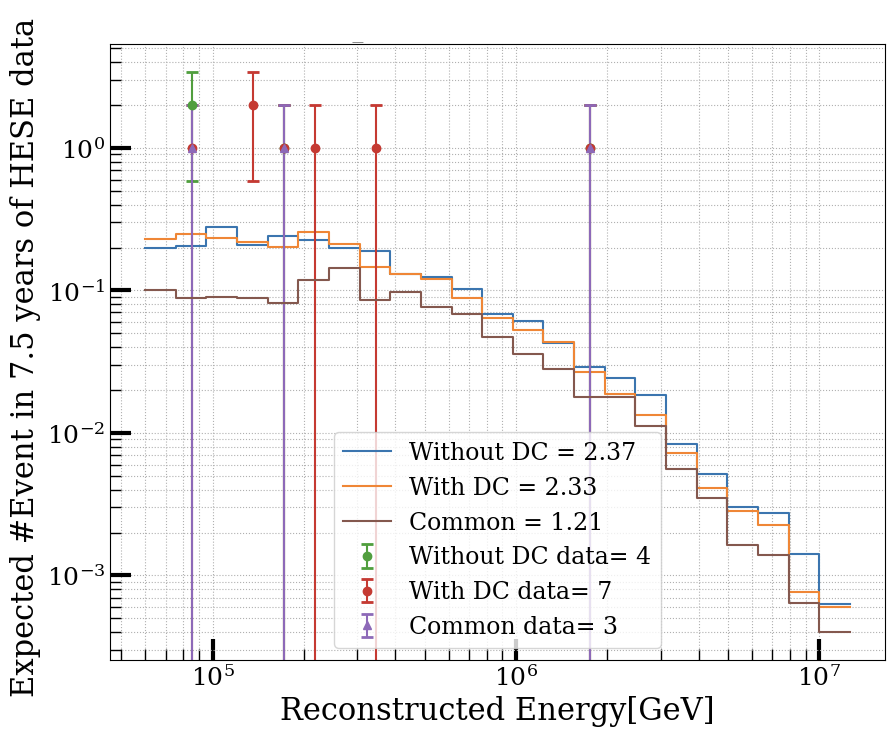
\includegraphics{./figures/results/Spice_DCwithdata.png}
    \end{subfigure}
    \hfill
    \begin{subfigure}[h]{0.7\textwidth}
        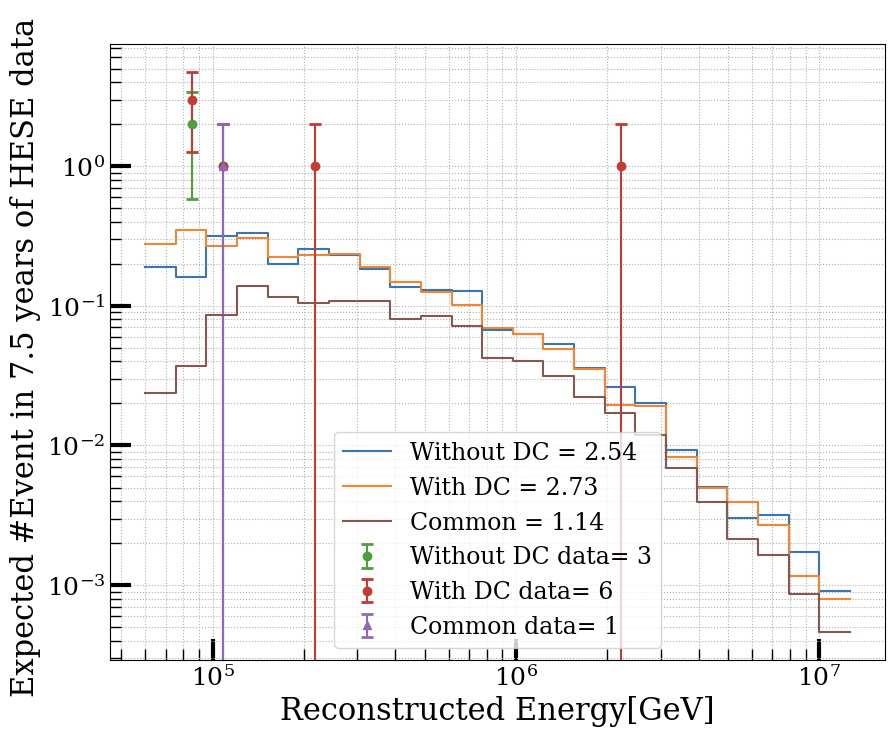
\includegraphics{./figures/results/Bfr_DCwithdata.png}
       
    \end{subfigure}%
    \caption[Data/MC distribution of HESE-7.5, using Spice-3.2.1 and Spice-Bfr icemodels, with and without DeepCore DOMs]{The Distribution of the expected number of events classified as double cascades in 7.5 years of HESE data, using the SPICE-3.2.1 (left) and SPICE-Bfr (right) ice models, with DeepCore(\emph{With DC}) and without DeepCore (\emph{Without DC}), along with the data events for each respective configuration.}
    \labfig{Bfr_DCwithdata}
\end{figure*}

\begin{table*}[h]
    \caption[Event classification of 7.5 years of HESE data, compared with reanalysis done using different ice models and inclusion/exclusion of DeepCore DOMs in the analysis]{Event classification of 7.5 years of HESE data (Previous) compared with reunblinded sample outcome (all events have Reconstructed total energy > 60 TeV ). The comparison is shown for all 2 different ice models, each of which further broken down into with and without the deepcore doms. The SPICE-BFR / No DeepCore configuration was selected for application to the full sample.}
    \labtab{HESE7_eventcomparisons}
    \raggedright
    \begin{tabular}{ c|c|c c |cc}
        \toprule
            & & \multicolumn{4}{c}{Reunblinded}\\
            
           Morphology&Previous & \multicolumn{2}{c|}{SPICE-3.2.1} & \multicolumn{2}{c}{SPICE-Bfr}\\
           
                     &   & DeepCore & No DeepCore & DeepCore & No DeepCore\\
                                
        \hline
        Cascades & 41 & 41 & 44 &42&45 \\
        Double Cascades & 2 & 7 &4&6& 3 \\
        Tracks& 17&14&14&16&14\\
        \hline
        Total & 60 & 62 &62&64&62\\
        \bottomrule
\end{tabular}
\end{table*}
\reffig{Bfr_DCwithdata} shows the distribution of classified Double Cascade, both with and without the inclusion of DeepCore DOMs. The Monte Carlo simulations predicts only 2-3 Double Cascade events, yet the data revealed 6 (7) Double Cascade events using SPICE-Bfr (SPICE-3.2.1) when DeepCore DOMs were included and only 3 (4) when they were excluded. It remains clear that for both ice models, the distribution of reconstructed energy and overall expectation remains same irrespective of whether DeepCore DOMs are included or not. This discrepancy pointed to potential issues in reconstruction processes involving DeepCore DOMs upon investigation. The \texttt{millipede} reconstructions, as explained in Section~\ref{sec:reco} relies on table-based light yield to quantify observed charge into photons, to account for deposited energies. To do this, it relies on Single Photoelectron (SPE) templates that are associated with each DOM. These templates were re-caliberated recently by using Flasher LEDs \sidecite{SPE_paper}, which saw a significant shift from the previously assumed mean value of this distribution for both DeepCore and Non-DeepCore DOMs. These updated templates had been used in simulations, but the change had not made its way through the calibration files used in data files (see Appendix~\ref{ch:spe_check} for details.). While the Non DeepCore DOMs' shift (<5\%) could be fixed via inclusion of optical efficiency parameter ($\eta_{\mathrm{domeff}}$) in the fit, the High QE DeepCore DOMs that showed >15\% difference could not rely on a nuisance parameter.  

All of these findings indicated that further investigation at the Monte Carlo level is necessary,  Such investigations requires efforts that were beyond the timeline of this thesis work and  considering the historical exclusion of DeepCore DOMs (as well as other "bad" DOMs such as bright or saturated modules) from reconstruction chains in previous iterations of HESE analyses, this analysis ultimately decided not to include DeepCore DOMs in the full sample unblinding. \textbf{By reconstructing data events using SPICE-Bfr ice model, without the DeepCore DOMs}, the re-anlaysis of the HESE-7.5 data resulted in 62 events with deposited energies above 60 TeV. Of these, 45 were classified as single cascades, 3 as Double Cascades, and 14 as track events. A detailed comparison between these  reunblinded results and previous results, including classified morphologies (with different iterations of ice models and DeepCore inclusion/exclusion) is shown in \reftab{HESE7_eventcomparisons}.

\section{Unblinding of 12 years of HESE data}
\label{sec:HESE12}
The High-Energy Starting Events (HESE) sample, covering approximately 12 years of IceCube detector live time (4268.7 days) from May 2010 to August 2022, was unblinded in January 2024 for the analysis outlined in Section 4.3. This sample includes 167 events that passed the HESE selection criteria, which involved the veto and total charge conditions as detailed in Section 4.2. Of these, 3 were coincident events that had previously been removed by manual inspection, but were retained this time since the current Monte Carlo simulations now account for such coincidences. Despite this, the energy threshold of 60 TeV effectively filtered them out, resulting in a final sample of 97 events above the 60 TeV deposited energy threshold. Using the ternary topology identification method from this thesis, 64 events were classified as single cascades, 5 as double cascades, and 28 as tracks.

\subsection{Fit results}
\label{sec:HESE12_fitresults}

\subsubsection{Blind Fit results}
\label{blindfit}
In IceCube, all the analysis are done in a blind fashion, meaning, all expected signal and background components for this search are modeled through simulation, which is then used to develop reconstruction algorithms, event selection criteria, and analysis frameworks. Before looking at the full results, a middle step was considered where only nuisance parameters of the fit were revealed first to identify potential striking disagreement between the data and Monte Carlo or unexplainable behaviour of any nuisance parameters (e.g. if they are hitting the boundary of the fit range), called \emph{the blind fit}. To reduce reliance on priors (as priors can penalize the likelihood as discusses in Section~\ref{sec:MLE}), this strategy of performing a blind fit was employed to identify nuisance parameters that require (pre-defined) priors due to their lack of constraints from the data. In addition, the goodness of fit was observed, the p-value of which was to be at least 5\%. The best fit values of nuisance parameters are summarized in \reftab{bf_nuisance} along with their gaussian priors. Most of the nuisance parameters fit to their base values (with a likelihood profile that reflects the prior). The detector systematics are not exactly fitting to theirdefault values, but they still remain within one standard deviation of the applied prior width.

\begin{figure}[ht]
	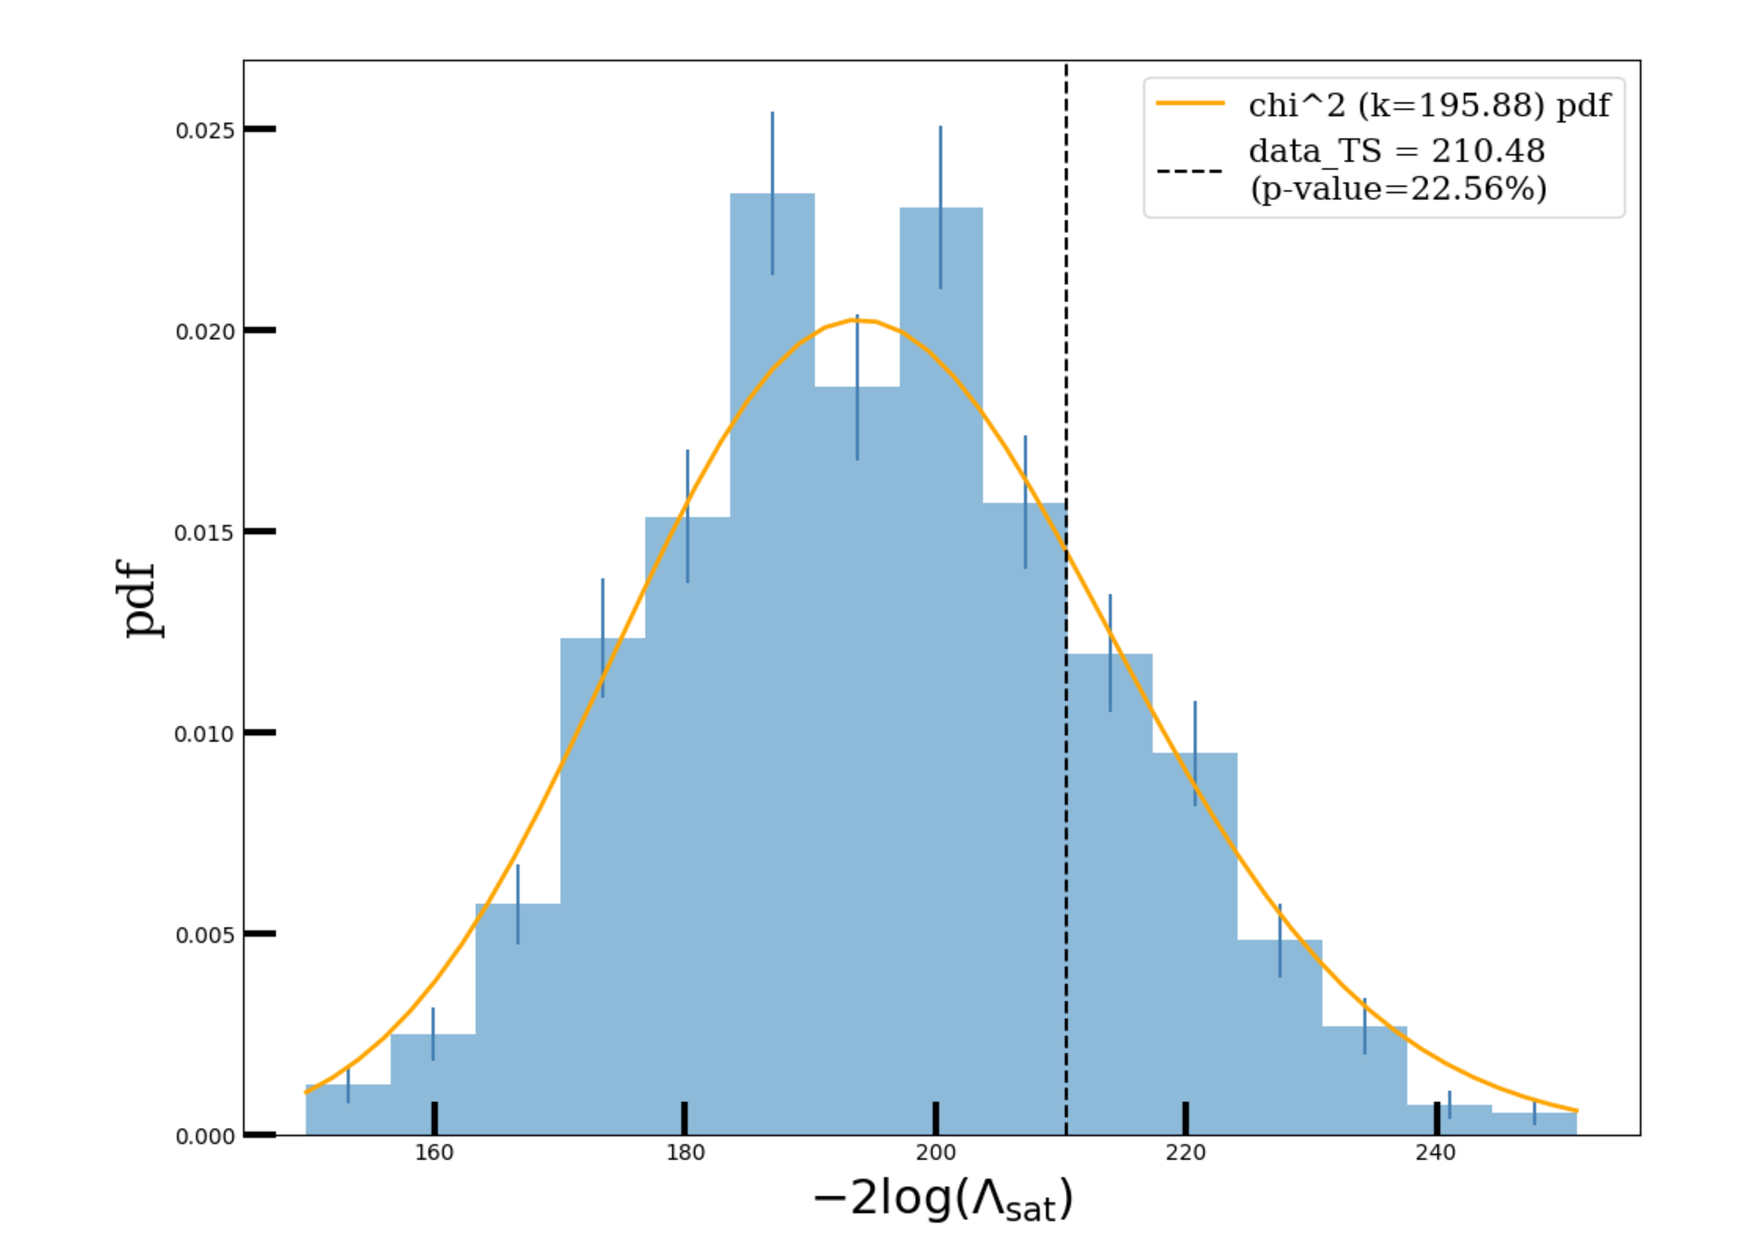
\includegraphics[scale=0.5]{./figures/results/GOF.pdf}
	\caption[GOF test for HESE-12]{Distribution of the test statistics for 1000 pseudotrials injected at best fit (signal parameters kept blind). Veritcal line shows TS of data, which matches quite well with degrees of freedom derived by fitting a $\chi^2$ to the distribution.}
    \labfig{gof}
\end{figure}

 
\begin{table*}[h]
    \caption[The best fit parameter values of the nuisance parameters in HESE-12 flavour fit]{The best fit parameter values of the nuisance parameters. The uncertainties are calculated at the 68\% confidence level through a profile likelihood scan assuming Wilks' theorem \cite{Wilks_thm}, in case of a flat likelihood space, fit boundaries are given as limits. Last column states the gaussian priors on the parameters (if applicable) in terms of the mean ($\mu$) and width ($\sigma$). The table is divided in terms of type of the nuisance parameters, above part includes all the parameters that affects the atmosphgeric neutrino components and the lower part consists if parameters stemming through various detector components. For details, see \ref{sec:params}}
    \labtab{bf_nuisance}
    {\renewcommand{\arraystretch}{1.4}
    \begin{tabular}{ c c |c|c}
        \hline
        \multicolumn{2}{c|}{Parameter}  & best fit value & Prior ($\mu,\sigma$)\\
        \hline
        \hline
        $\Phi_{\mathrm{conv}}$& Conventional Flux normalisation & $0.99_{-0.2}^{+0.19}$ & (1.0,0.2)\\
        \hline
        $\Phi_{\mathrm{prompt}}$& Prompt Flux Normalisation & ${0.0}_{-0.0}^{+2.25}$ & - \\
        \hline
        $\xi_{\mathrm{CR}}$& Interpolation between Cosmic Ray Models & $0.042_{-1}^{+2}$ & (0,1)\\
        \hline
        $\Delta\gamma_{\mathrm{CR}}$& Cosmic Ray Spectral Index Shift & $-0.00_{-1}^{+1}$ & (0,0.05)\\
        \hline
        $H_{\mathrm{Barr}}$& Barr-parameter modifying the pion-contribution & $0.0_{-0.5}^{+0.5}$ & (0,0.15)\\
        \hline
        $W_{\mathrm{Barr}}$& Barr-parameter modifying the kaon-contribution & $0.0_{-0.5}^{+0.5}$ & (0,0.40)\\
        \hline
        $Y_{\mathrm{Barr}}$& Barr-parameter modifying the pion-contribution & $0.0_{-0.5}^{+0.5}$ & (0,0.30)\\
        \hline
        $Z_{\mathrm{Barr}}$& Barr-parameter modifying the pion-contribution & $0.0_{-0.5}^{+0.5}$ & (0,0.12)\\
        \hline
        $\Phi_{\mathrm{muongun}}$ & Muon Flux Normalisation & $1.16_{-0.43}^{+0.42}$ & (1,0.5)\\
        \hline
        $\mathrm{I}_{\mathrm{scale}}$ & scale factor for Neutrino Nucleon Inelasticity weight & $0.99_{-0.09}^{+0.1}$ & (1,0.1)\\
        \hline
        
        \multicolumn{4}{c}{\textbf{Detector Systematics}}\\
        \hline
        $\eta_{\mathrm{domeff}}$& Optical Efficiency of DOMs & $1.04_{-0.04}^{+0.06}$ & (1.0,0.1)\\
        \hline
        $\eta_{\mathrm{abs}}$& Ice Absorption Scaling & $0.99_{-0.04}^{+0.04}$ & (1.0,0.05)\\
        \hline
        $\eta_{\mathrm{scat}}$& Ice Scattering Scaling & $0.98_{-0.04}^{+0.04}$ & (1.0,0.05)\\
        \hline
        $\eta_{\mathrm{h.ice-p0}}$& parametrization for refrozen icecolumn & $-0.27_{-0.38}^{+0.28}$ & (-0.27,0.5)\\
        \hline
        $\eta_{\mathrm{h.ice-p1}}$& parametrization for refrozen icecolumn & $-0.08_{-0.05}^{+0.04}$ & (-0.042,0.05)\\
        \hline
        $\eta_{\mathrm{aniso}}$& Ice Anisotropy Scaling & $0.99_{-0.63}^{+0.54}$ & -\\
        \hline
        \hline
    \end{tabular}
    }
\end{table*}

Lastly, the goodness of the fit (GOF) is tested by using using the pseudo data samples. This data is generated by populating the analysis histograms by drawing the number of events in each bin from a Poisson distribution with the mean given by  simulation expectations for this bin at the best fit parameter values. These pseudo-data samples are then analyzed in the same way as ther real data to obtain a distribution of test statistic values from the outcomes. The saturated model is the one where the data is the model, i.e. the expectation for each bin is the observed counts. Where each analysis bin observes statistically significant data, following a $\chi^2$ distribution with degrees of freedom equal to the difference between the number of analysis bins and the number of free parameters in the fit. However, in reality, not all bins observe data, so some deviations are expected. By comparing the distribution of TS values from these pseudo-data trials to the distribution derived from the real data, a p-value can be calculated. The p-value represents the probability of finding a TS value from the trials that is at least as large as the one from the data fit. \reffig{gof} illustrates this distribution, where the data TS is compared with the distribution of trial TS values. The obtained p-value is 22.56\%. Based on this test, it is concluded that the fit result is consistent with the expected outcome from the pseudo-data trials.


\subsubsection{Full fit results}
\label{final_fit}
In this section, we discuss the full results, i.e signal parameters of the fit performed. The best fit values of the signal parameters for the 97 HESE events are summarized in \reftab{bf_signal}. As explained in \ref{sec:params}, the flavour fractions within \texttt{NNMFit} framework are fitted as scaling factors $s_{\nu_{e}}$ and $s_{\nu_{\tau}}$, which modifies the flux of electron and tau neutrinos relative to the muon neutrino flux. Which is why, the signal parameters listed in \reftab{bf_signal} needs to be converted to their corresponding flavour fractions (by using Equation~\ref{eq:flav_frac}), yielding a best fit flavour composition of astrophysical neutrinos as, \textbf{$f_{\nu_e}:f_{\nu_{\mu}}:f_{\nu_{\tau}} = 0.19_{-0.15}^{+0.26}:0.43_{-0.17}^{+0.27}:0.38_{-0.24}^{+0.37}$}.

\begin{table*}[h]
    \caption[The best fit parameter values of the signal parameters in HESE-12 flavour fit]{The best fit signal parameters for a single power-law model for both particle and antiparticle. The uncertainties are calculated at the 68\% confidence level through a profile likelihood scan assuming Wilks' theorem.}
    \labtab{bf_signal}
    {\renewcommand{\arraystretch}{1.4}
    \begin{tabular}{ c c |c}
        
        \hline
        \multicolumn{2}{c|}{Parameter}  & best fit value\\
        \hline
        \hline
        $\phi_{\nu_{\mu}}$ &astro. $\nu_{\mu}$ normalisation [$10^{-18} \mathrm{GeV}^{-1}\mathrm{cm}^{-2}\mathrm{sr}^{-1}\mathrm{s}^{-1}$]& $2.53_{-1.49}^{+1.78}$\\
        \hline
        $\gamma_{\mathrm{astro}}$ &astro. spectral index & $2.84_{-0.18}^{+0.19}$\\
        \hline
        $s_{\nu_e}$ &astro. $\nu_{e}$ scaling factor to modify total flux norm ($\Phi_{\nu+\bar\nu}^{\mathrm{astro}}$) relative to $\phi_{\nu_{\mu}}$ & $0.45_{-0.40}^{+0.68}$\\
        \hline
        $s_{\nu_{\tau}}$ &astro. $\nu_{\tau}$ scaling factor to modify total flux norm ($\Phi_{\nu+\bar\nu}^{\mathrm{astro}}$) relative to $\phi_{\nu_{\mu}}$ & $0.896_{-0.89}^{+1.34}$\\
        \hline
        \hline
    \end{tabular}
    }
\end{table*}


The best fit value of astrophysical index ($\gamma_{\mathrm{astro}}$), assuming a single power law is $2.84_{-0.18}^{+0.19}$. This value is in well agreement with the previous results \sidecite{HESE7_sample}. The  normalization of the all-flavour neutrino flux derived from the fit result is $\Phi_{\nu+\bar\nu}^{\mathrm{astro}} = 5.94_{-4.28}^{+5.64}$. Te larger uncertainity on normalization is expected for such a fit where each flavour components are allowed to be free, that in turn have larger uncertainty on them (see \reftab{bf_signal}). 

Lastly, the table in \reftab{pid_comparisons} provides the breakdown of expected events classified into specific morphologies and their individual components for the best fit model. Additionally, the comparison includes the expectation based on a $f_{\nu_e}:f_{\nu_{\mu}}:f_{\nu_{\tau}} = 1:1:1$ flavour ratio, which was determined by running the fit with fixed flavour ratios.

\begin{table*}[h]
    \caption[The expected number of HESE events in 12 years at the best fit value]{The expected number of HESE events, classified into three morphologies, assuming a fixed flavour ratio of 1:1:1 and at the best fit flavour ratio. The total expected event counts are further broken down into each of the flux components, Astrophysical (Astro), Conventional atmospheric neutrinos (Conv), Atmospheric Muons (Muon). Prompt atmopsheric neutrino component is not shown here as best fit value of the prompt norm ($\Phi_{\mathrm{prompt}}$) is 0.}
    \labtab{pid_comparisons}
    
    \begin{tabular}{ c| c c c c |c c c c|c}
        
        \hline
        \makecell{Reconstructed \\ Morphology} & \multicolumn{4}{c|}{$f_{\nu_e}:f_{\nu_{\mu}}:f_{\nu_{\tau}} = 1:1:1$(fixed)}  & \multicolumn{4}{c|}{$f_{\nu_e}:f_{\nu_{\mu}}:f_{\nu_{\tau}} = 0.19:0.43:0.38$ (free)} & Data\\
         &Astro&Conv&Muon&Total&Astro&Conv&Muon&Total& \\
        \hline
        \hline
        Cascades&$58\pm2$&$6.8\pm0.9$&-&\textbf{$65\pm2.7$}&$57\pm2$&$6\pm0.79$&-&\textbf{$63.4\pm2.4$}&\textbf{64}\\
        Tracks&$11.8\pm0.7$&$6.3\pm1$&$2\pm3$&\textbf{$20\pm3.6$}&$16\pm0.8$&$5.7\pm0.9$&$1.84\pm2.7$&\textbf{$23.4\pm3.4$}&\textbf{28}\\
        \makecell{Double \\ Cascades}&$3.2\pm0.3$&$0.4\pm0.2$&-&\textbf{$3.5\pm0.5$}&$3.8\pm0.3$&$0.3\pm0.2$&-&\textbf{$4.1\pm0.4$}&\textbf{5}\\
        \hline
        \hline
    \end{tabular}
    
\end{table*}

\subsection{Data/Monte Carlo Agreement}
\label{sec:data_mc}
In addition to the goodness-of-fit test, comparisons of data with Monte Carlo expectations for a few key parameters were performed. \reffig{Cascades_datamc}, \reffig{Tracks_datamc} and \reffig{double_datamc} shows the distributions of the analysis observables for all three morphologies, for HESE events with deposited energies above 60 TeV. These plots are generated using the best fit values stated in \reftab{bf_signal} and \reftab{bf_nuisance}. Each figure displays individual components as well as the sum of all components under the label \textbf{MC sum}. Additionally, to highlight any noteworthy features, a ratio plot is included for each distribution, illustrating the ratio of data events to each bin of the total number of expected simulation events. Due to the low number of observed events, it is challenging to pinpoint any specific spectral features, that these distributions may exhibit. 

\reffig{Cascades_datamc} and \reffig{Tracks_datamc} shows the distribution of reconstructed energy (left) and cosine of reconstructed zenith (right) for events classified as single cascades and tracks resepctively in the 12 years of HESE data. The zenith plot clearly illustrates the all-sky coverage of the HESE sample as events are observed across the zenith range. It also highlights the decrease of the conventional component in the downgoing region (cos(zenith>0.25)), indicating the self-veto effect (described in Section~\ref{sec:selfveto}). Additionally, the atmospheric muongun component is exclusively visible in the track histogram since muons produce track-like events. However, it's important to note that the expectation exhibits substantial statistical uncertainties due to the lack of sufficient \texttt{muongun} Monte Carlo\sidenote{this lack of simulation is due to the immense amount of computing time that is needed to produce single muons that reach the detector at such high energies.}. To mitigate the impact of statistical fluctuations caused by the low number of simulated events, a kernel density estimation (KDE) is employed to smoothen out the distribution. 

\begin{figure*}[h]
    \begin{subfigure}[h]{0.7\textwidth}
        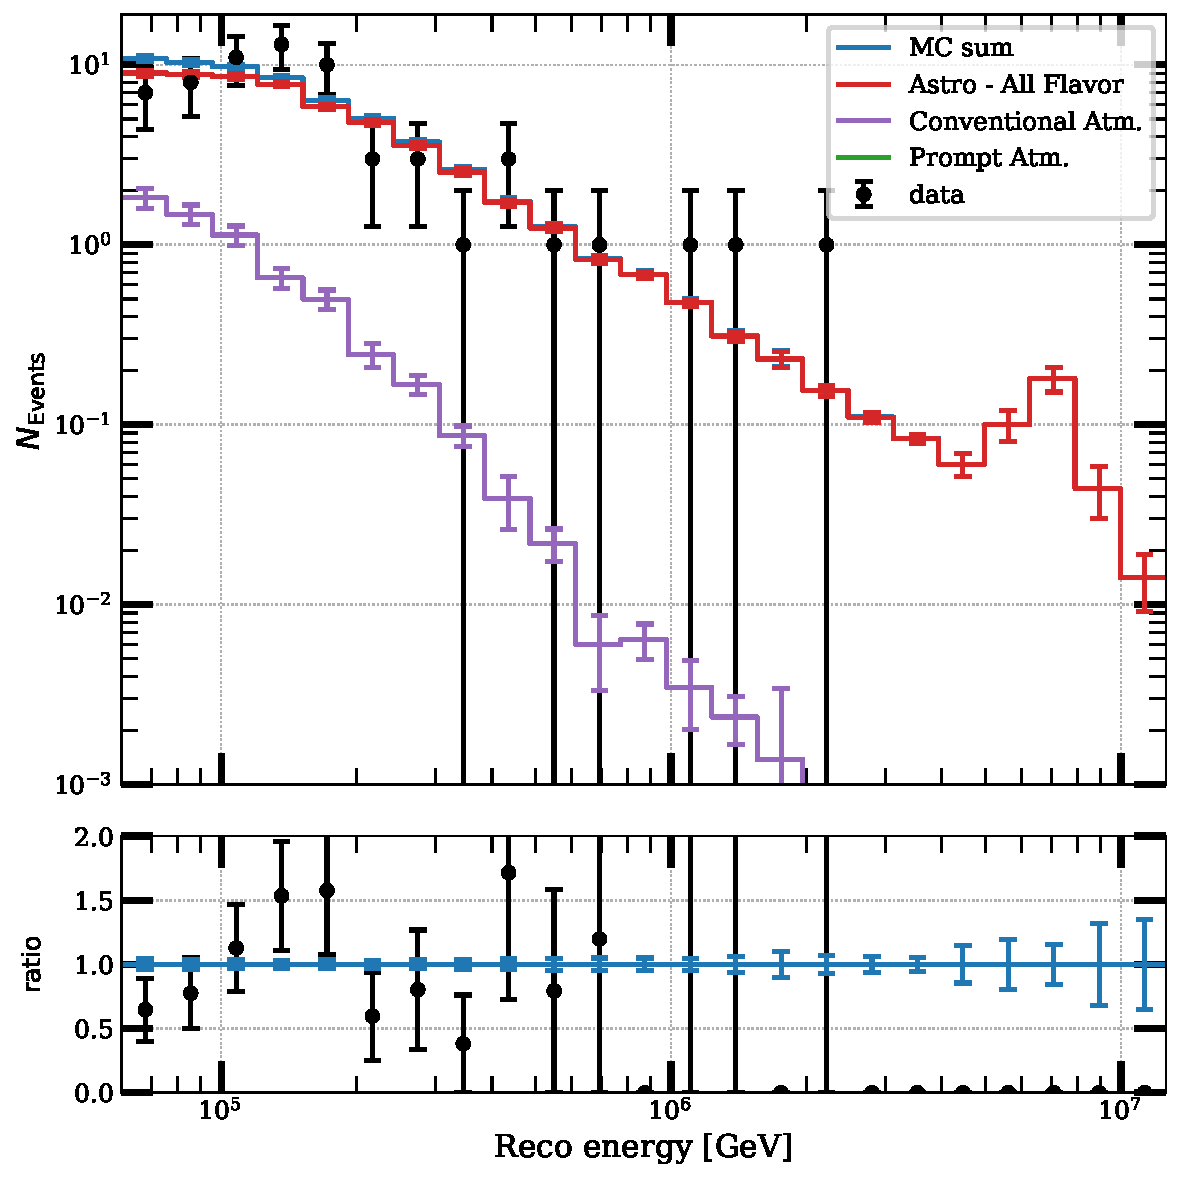
\includegraphics{./figures/results/DataMC_IC86_pass2_SnowStorm_v2_Bfr_Cascades_energy.pdf}
    \end{subfigure}
    \hfill
    \begin{subfigure}[h]{0.7\textwidth}
        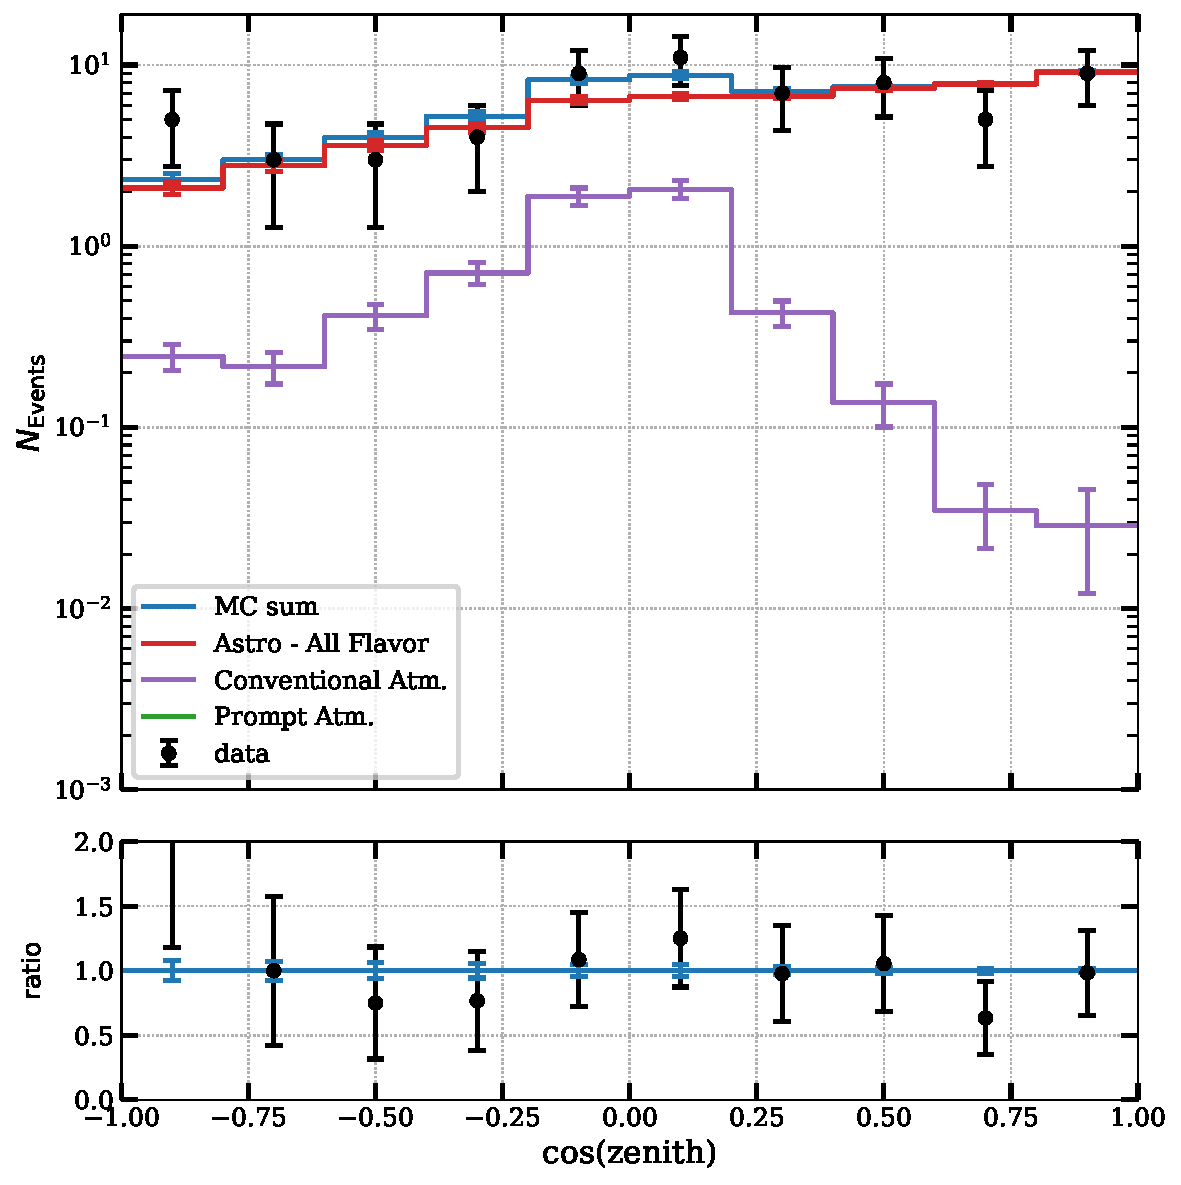
\includegraphics{./figures/results/DataMC_IC86_pass2_SnowStorm_v2_Bfr_Cascades_zenith.pdf}
       
    \end{subfigure}%
    \caption[Data/MC agreement for HESE-12 Cascades]{Distributions of the total reconstructed deposited energy (left) and the zenith angle (right) for events classified as \textbf{single cascades} along with data point positions. Individual components of the fits are produced using best fit values given in \reftab{bf_signal} and \reftab{bf_nuisance} and "MC sum" labels the sum of all of these components. The Prompt component is not shown on account of best fit value of 0 for the $\Phi_{\mathrm{prompt}}$.}
    \labfig{Cascades_datamc}
\end{figure*}

\begin{figure*}[h!]
    \begin{subfigure}[h]{0.7\textwidth}
        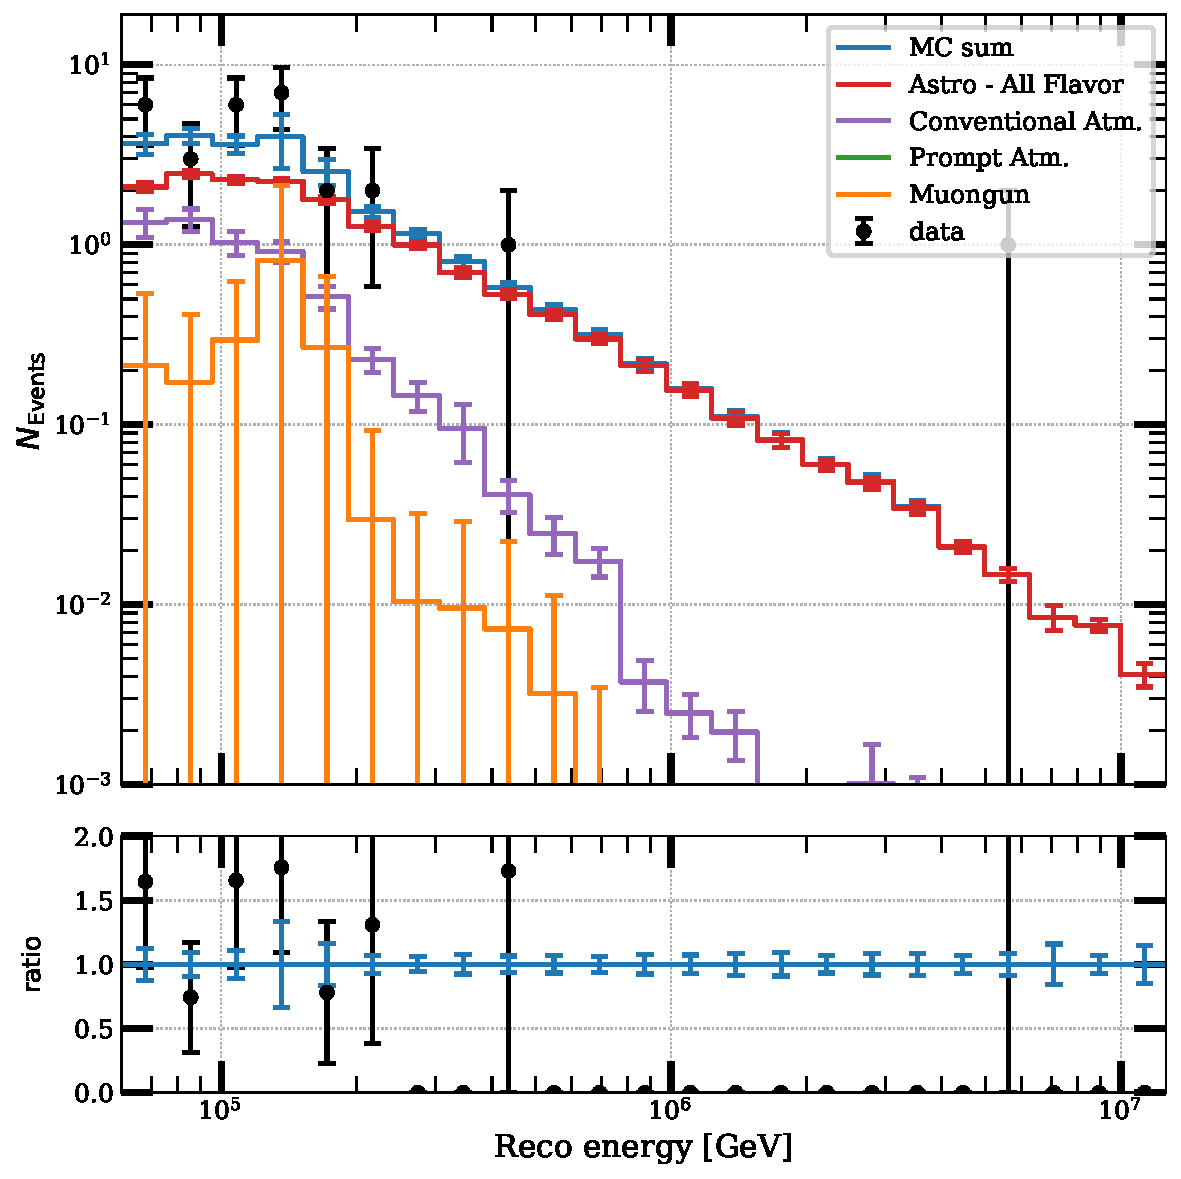
\includegraphics{./figures/results/DataMC_IC86_pass2_SnowStorm_v2_Bfr_Tracks_energy.pdf}
    \end{subfigure}
    \hfill
    \begin{subfigure}[h]{0.7\textwidth}
        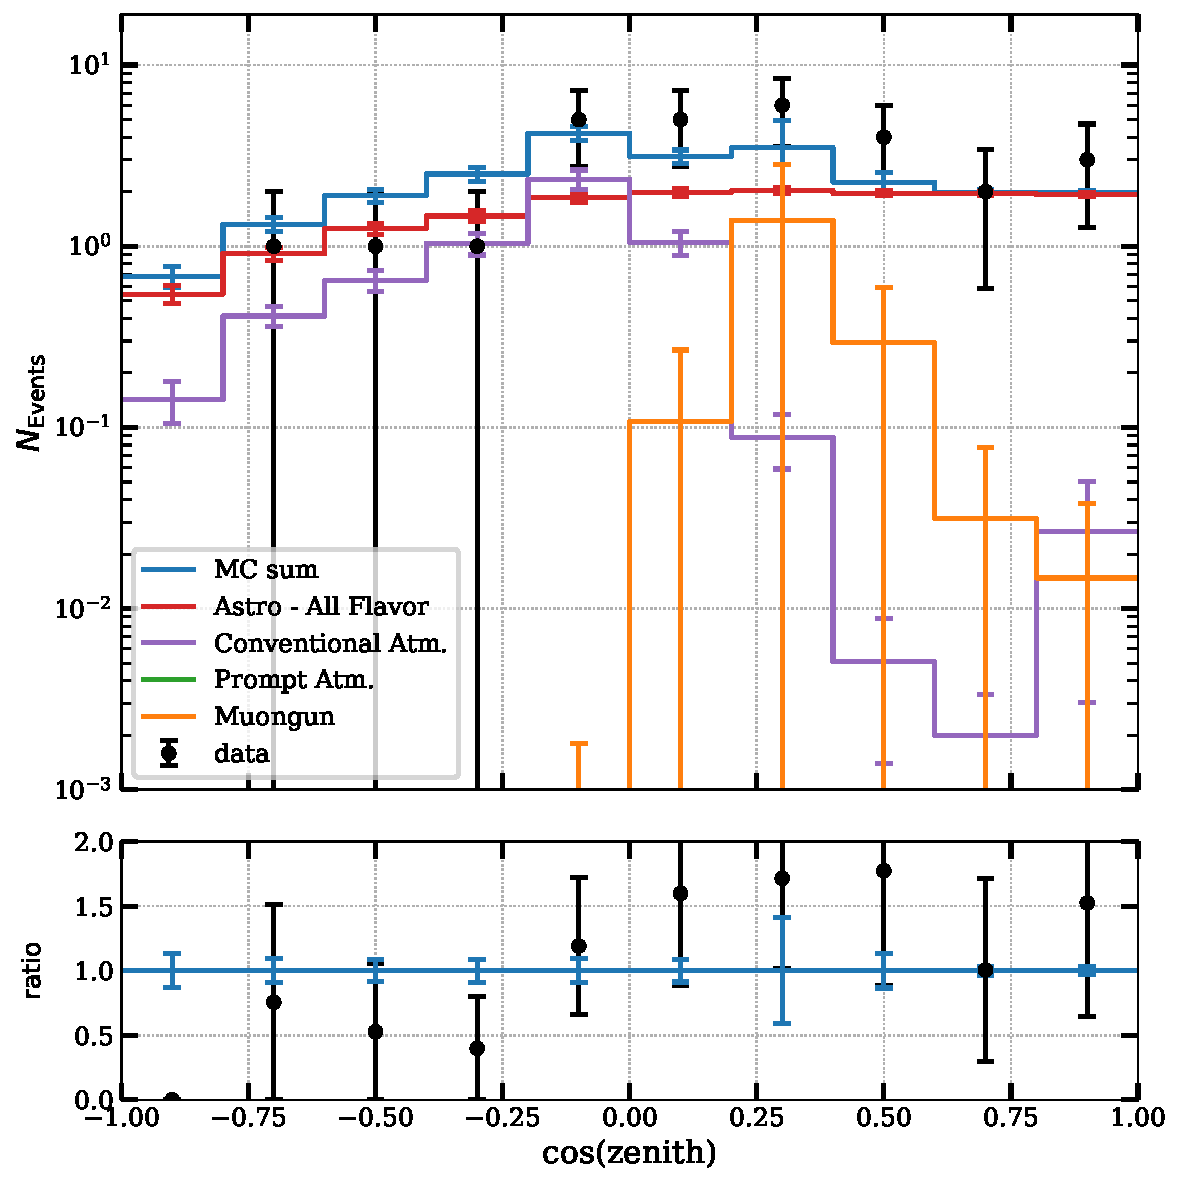
\includegraphics{./figures/results/DataMC_IC86_pass2_SnowStorm_v2_Bfr_Tracks_zenith.pdf}
       
    \end{subfigure}%
    \caption[Data/MC agreement for HESE-12 Tracks]{Distributions of the total reconstructed deposited energy (left) and the zenith angle (right) for events classified as \textbf{tracks} along with data point positions. Individual components of the fits are produced using best fit values given in \reftab{bf_signal} and \reftab{bf_nuisance} and "MC sum" labels the sum of all of these components. The Prompt component is not shown on account of best fit value of 0 for the $\Phi_{\mathrm{prompt}}$.}
    \labfig{Tracks_datamc}
\end{figure*}
\newpage
\reffig{double_datamc} illustrates the distribution of reconstructed energy (left) and reconstructed length (right) for events classified as double cascades in the 12 years of HESE data. The first two bins show in reconstructed energy show an overfluctuation while the rest of the histrogram is empty, but the interpretation is challenging due to the low number of involved events. A noteworthy observation is that one event, although close to 100 TeV, has a large length, suggesting that it is a misclassified track. This particular event demonstrates Energy Confinement near the cut boundary (0.991), a cut that is supposed to differentiate between a double cascade and a track, but not quite the threshold to be a track ($E_C<0.99$). And hence, the event passed all the cuts and ended up being classified as a double cascade. This becomes more evident in 2D distribution of energy and length in \reffig{LvsE_datamc}, where this event clearly ends up in a  background dominated region of the PDF (see \ref{sec:PID} for signal and background pdfs of double cascades). 


\begin{figure*}[h]
    \begin{subfigure}[h]{0.7\textwidth}
        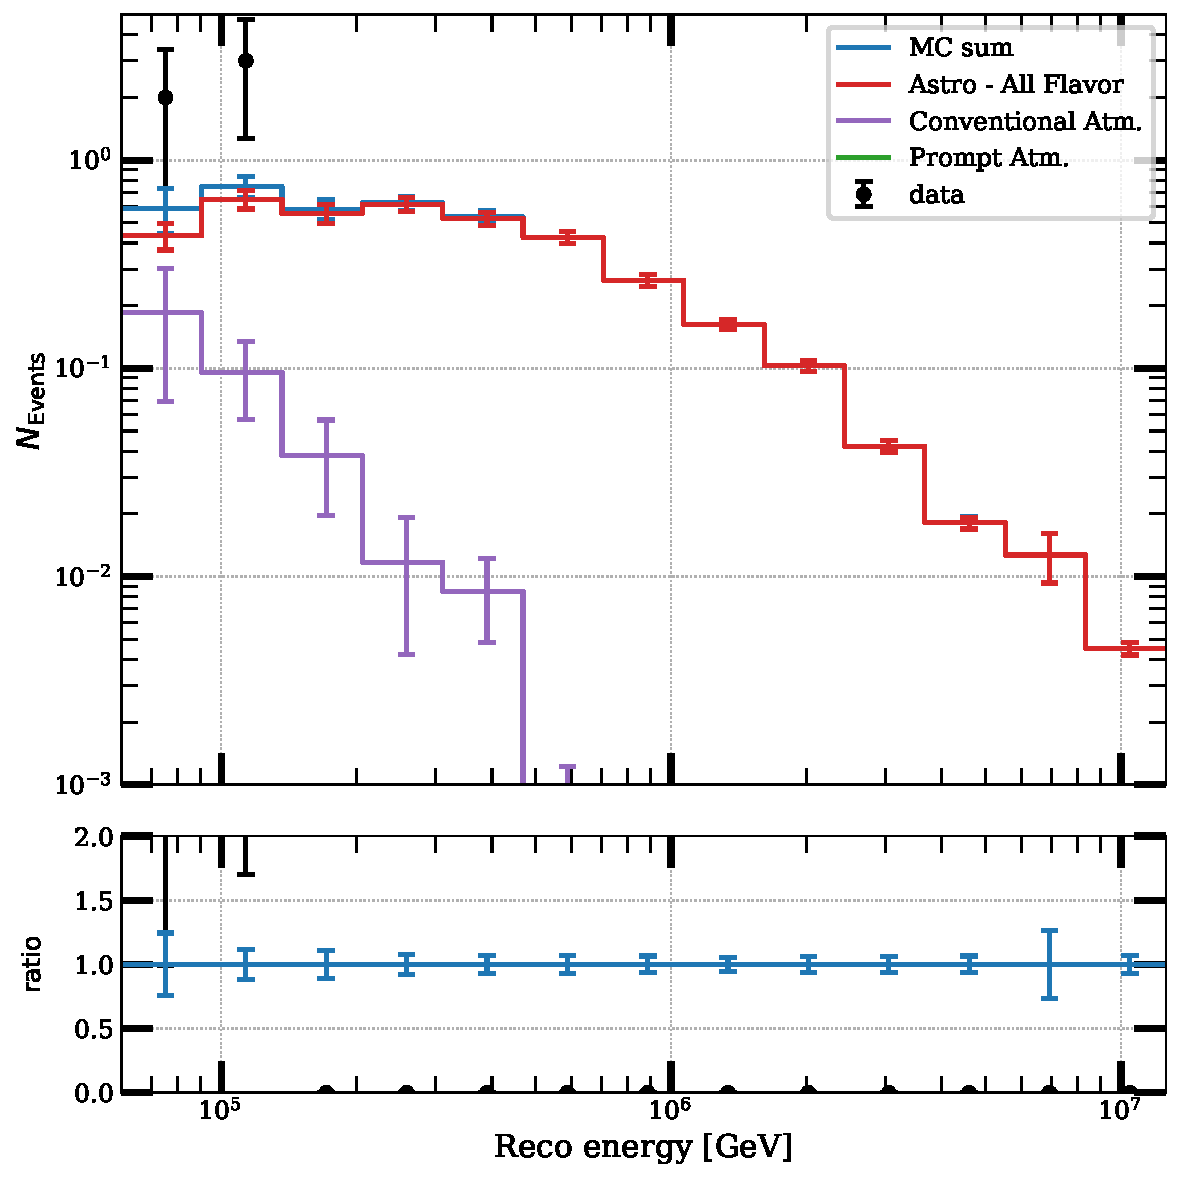
\includegraphics{./figures/results/DataMC_IC86_pass2_SnowStorm_v2_Bfr_DoubleCascades_energy.pdf}
    \end{subfigure}
    \hfill
    \begin{subfigure}[h]{0.7\textwidth}
        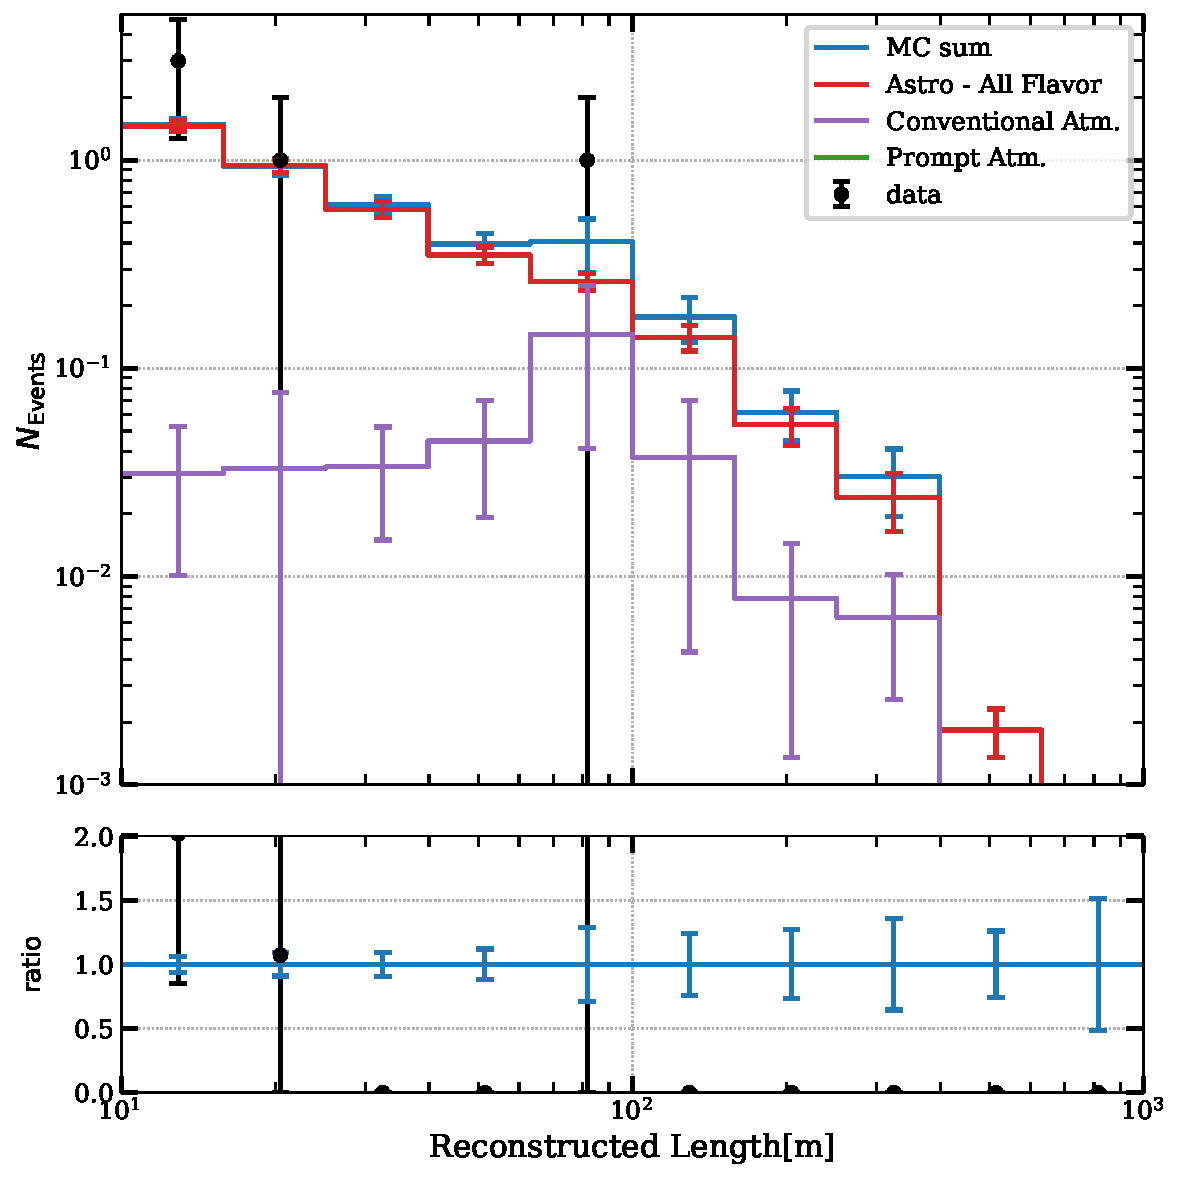
\includegraphics{./figures/results/DataMC_IC86_pass2_SnowStorm_v2_Bfr_DoubleCascades_zenith.pdf}
       
    \end{subfigure}%
    \caption[Data/MC agreement for HESE-12 Double Cascades]{Distributions of the total reconstructed deposited energy (left) and the zenith angle (right) for events classified as \textbf{double cascades} along with data point positions. Individual components of the fits are produced using best fit values given in \reftab{bf_signal} and \reftab{bf_nuisance} and "MC sum" labels the sum of all of these components. The Prompt component is not shown on account of best fit value of 0 for the $\Phi_{\mathrm{prompt}}$.}
    \labfig{double_datamc}
\end{figure*}
The \reffig{LvsE_datamc} illustrates a pdf for the energy and length distribution of events reconstructed as double cascades, based on the best fit values described in the tables. The vertical lines demonstrate how quickly the single-cascade background decreases with length. For instance, 68\% of misclassified single cascades have reconstructed double-cascade lengths of less than $\sim 14$ m, 90\% have lengths below $\sim  20$ m, and only 1\% have lengths exceeding $\sim 25$ m. Two of the data events are outside the 68\% region, but one of these events is still within the signal region indicated by white lines. The event with a reconstructed length of approximately 95 m but less than 80 TeV energy is clearly in the background region. Another important observation from this figure is the lack of smoothness expected from PDFs when performing forward folding fits. The gradients are applied as an additive correction per bin, to allow detector systematic variations in the fit. 
\begin{figure}[h]
    
    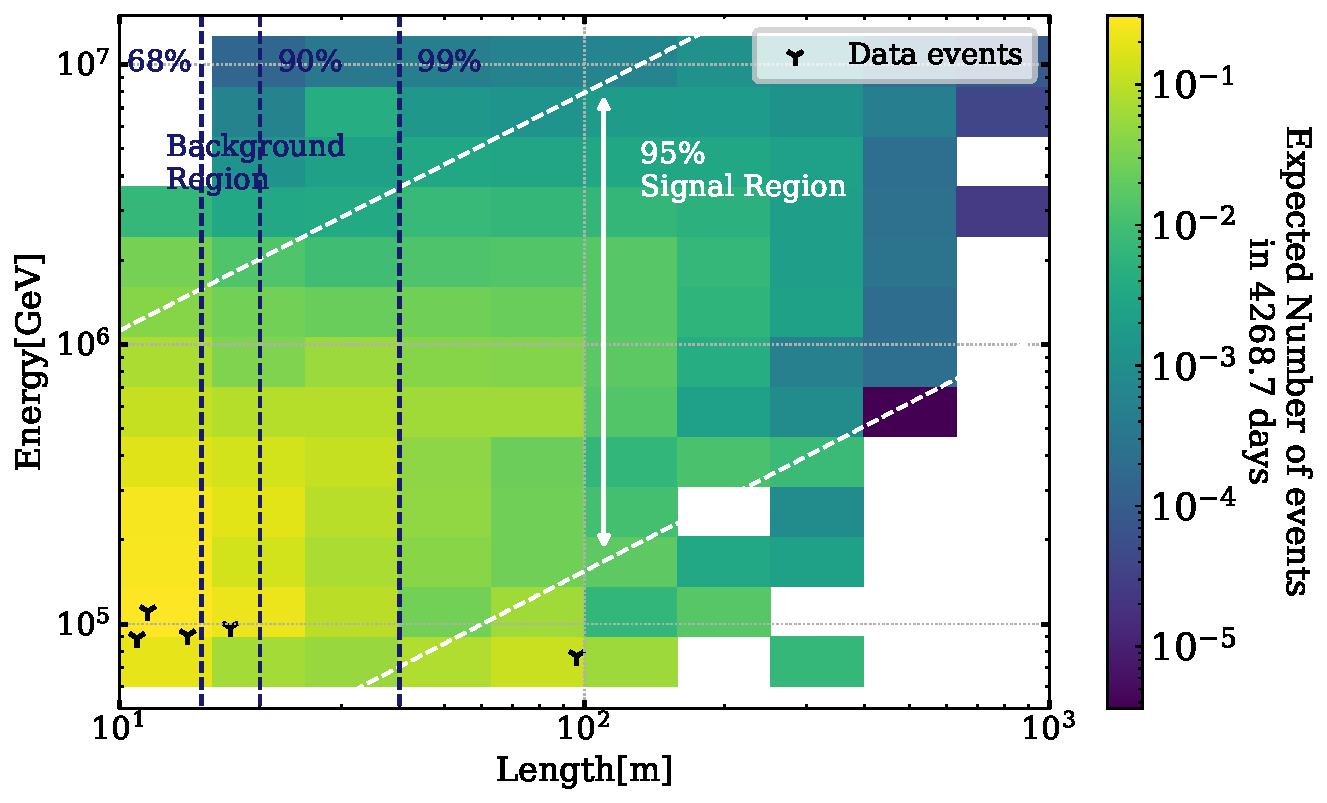
\includegraphics{./figures/results/DataMC_IC86_pass2_SnowStorm_v2_Bfr_DoubleCascadesLvsE_2D_withData.pdf}
    
    
    \caption[Two dimensional PDF of length vs Energy of double cascade sample at best fit showing data events positions]{Two-dimensional distribution of reconstructed energy vs reconstructed double cascade length of the Monte Carlo events classified as double cascades. Monte Carlo sum is produced using all the best fit parameters from the \reftab{bf_signal} and \reftab{bf_nuisance}. Position of the data events are marked with \wye[rotate=180]. Signal (white) and Background (dark blue) dominated regions are marked with their respective percentiles.}
    \labfig{LvsE_datamc}
\end{figure}

\begin{figure}
    
    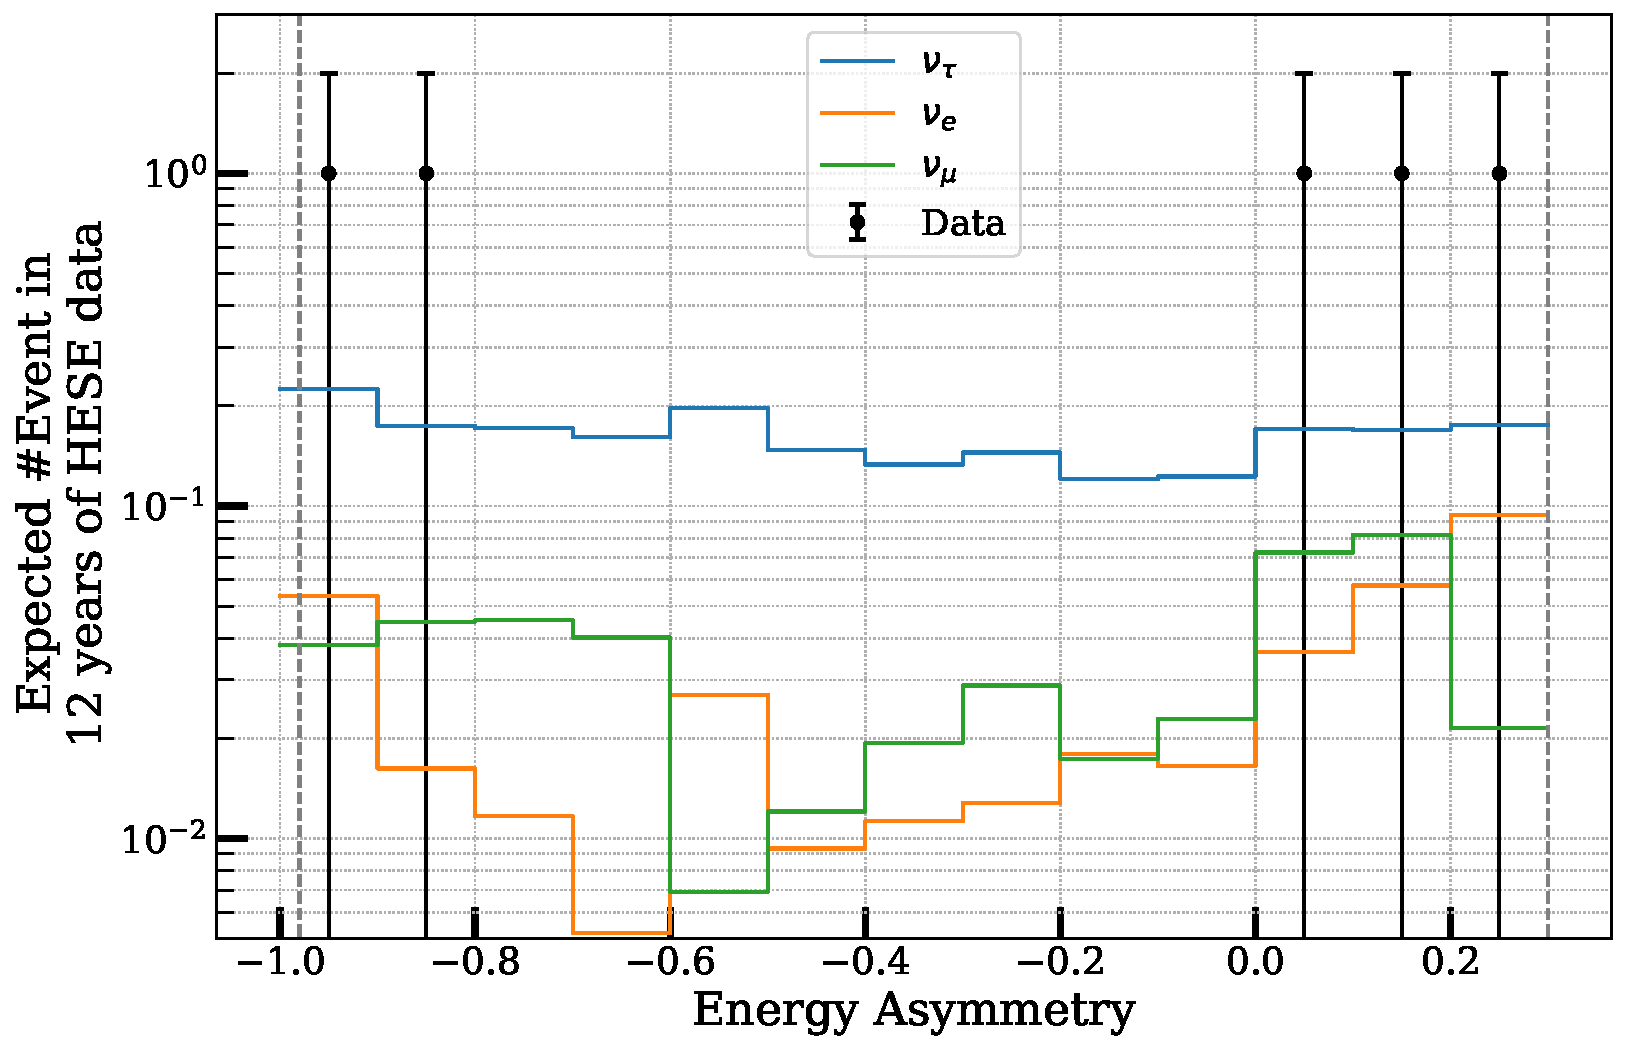
\includegraphics{./figures/results/Energy_ratio.pdf}
    
    \caption[Data/MC distribution of Energy asymmetry in double cascade sample]{Expected distribution of reconstructed energy asymmetry, defined as $\mathrm{E}_{\mathrm{A}}=\frac{\mathrm{E}_1-\mathrm{E}_2}{\mathrm{E}_1+\mathrm{E}_2}$, (where $\mathrm{E}_1$ and $\mathrm{E}_2$ are energies of first and second cascades, respectively) at best fit, along with data events. Distribution is shown for all flavours separately, to emphasis domination of $\nu_{\tau}$ double cascades in the signal region (verticla grey lines).}
    \labfig{Eratio}
\end{figure}

\reffig{Eratio} presents the distribution of the reconstructed energy asymmetry for simulated events in the double-cascade sample, using the best fit astrophysical and atmospheric spectra. The two vertical lines represent the selection cuts applied to choose the double cascade events, as described in section 4.3. Although two of the 5 events are near the cut edge, they all still fall comfortably within the signal-dominated region of the sample.

\section{Flavour Composition of Diffuse Astrophysical Neutrinos}
\label{sec:flavour_results}
The flavour composition of astrophysical neutrinos is measured using 97 high-energy starting event (HESE) events, which are divided among three morphologies. The profile likelihood scans for the flavour scale factors, specifically $s_{\nu_{e}}$ and $s_{\nu_{\tau}}$, are shown in \reffig{1d_llh}. The results indicate that the tau scale factor ($s_{\nu_{\tau}}$) is only able to reject the possibility of no $\nu_{\tau}$ flux by $1\sigma$, also reflected in the wide contours in the 2D scan shown in \reffig{flavour_comp}. The 1D scans are used to derive $1\sigma$ (68\%) confidence regions, shown in \reftab{bf_signal}. The test statistic $-2\Delta \log \mathcal{L}$ compares the global best fit values of the unconstrained fit to the conditional best fit values of all remaining model parameters at a fixed scan point. The confidence regions depicted in \reffig{flavour_comp} are calculated using Wilk's theorem \sidecite{Wilks_thm} , as a full Feldman-Cousins construction of the entire flavour composition phase space is computationally demanding (see section \ref{sec:analysis} for details). The applicability of Wilk's theorem is verified by comparing the coverage of the test statistic distribution from Monte Carlo pseudo-experiments to the coverage of a $\chi^2$-distribution, see Appendix~\ref{ch:wilks}. A large fraction of the flavour composition phase space is found to be slightly over-covered, indicating that Wilk's theorem yields a conservative confidence region. Although a part of the 90\% confidence region seems to suffer from slight under-coverage, the $\chi^2$-approximation is deemed sufficient for presenting the measurement result in \reffig{flavour_comp}. 

\begin{figure*}[h!]
    \begin{subfigure}[h]{0.7\textwidth}
        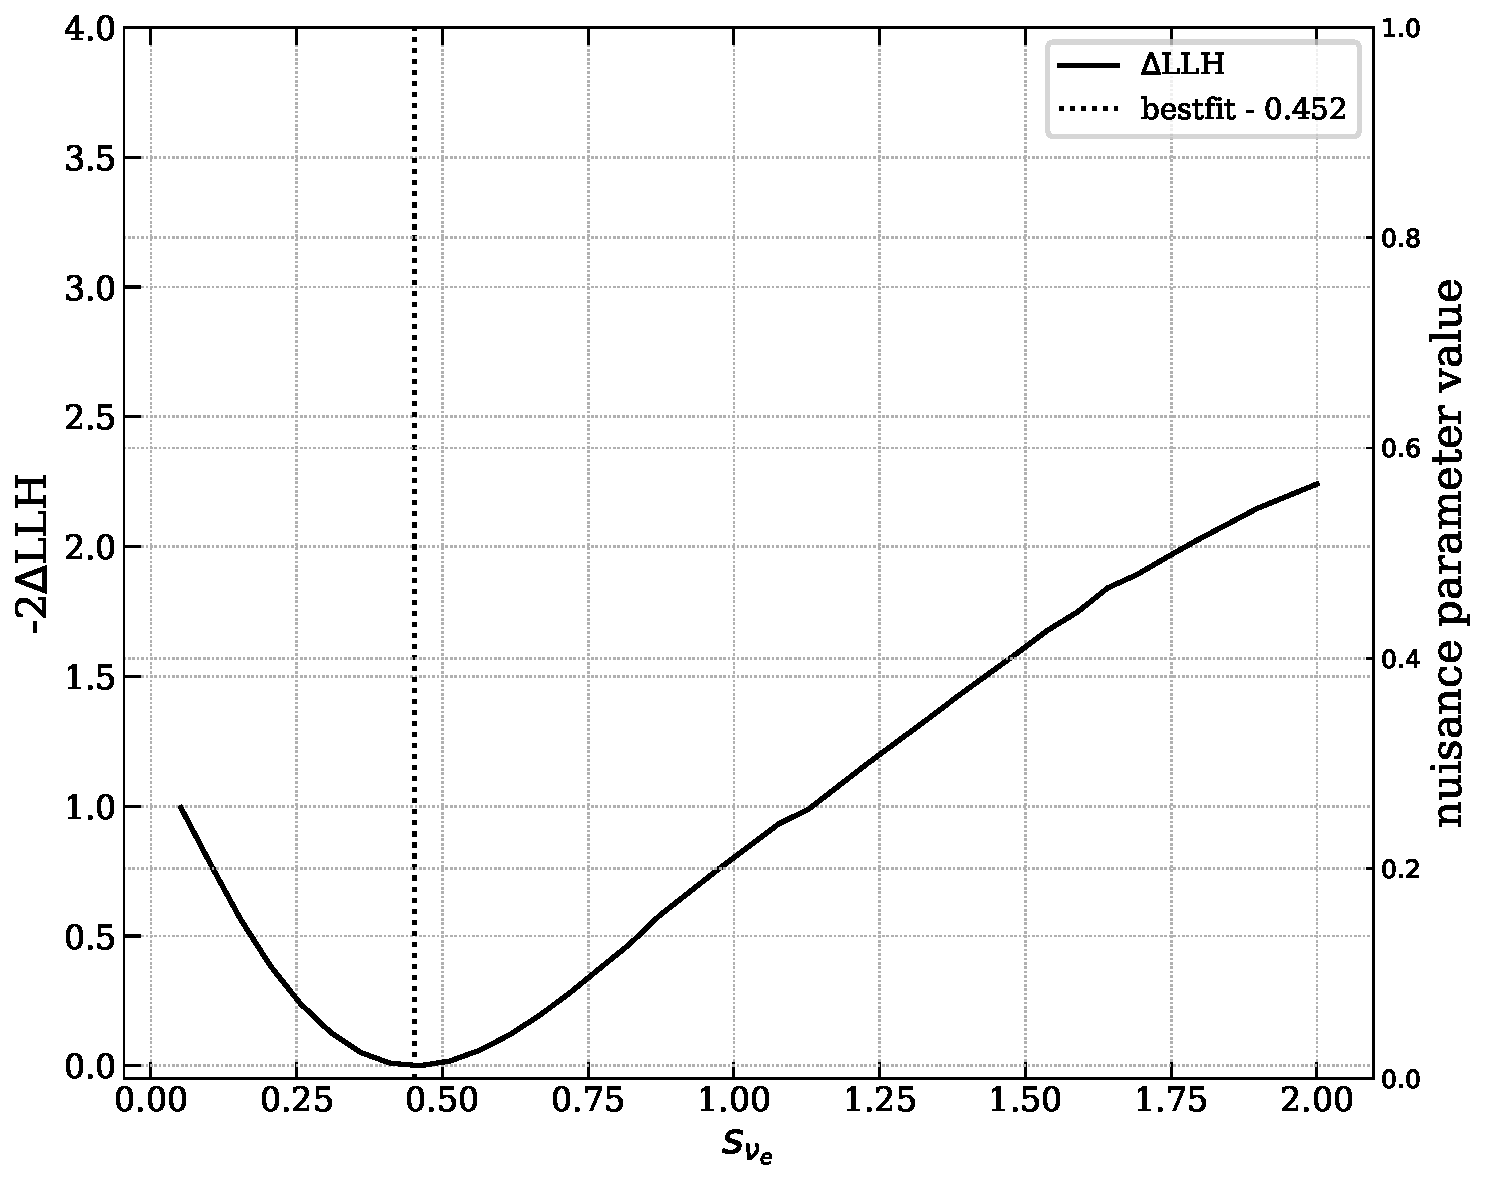
\includegraphics{./figures/results/profile_scan_astro_nue_ratio.pdf}
    \end{subfigure}
    \hfill
    \begin{subfigure}[h]{0.7\textwidth}
        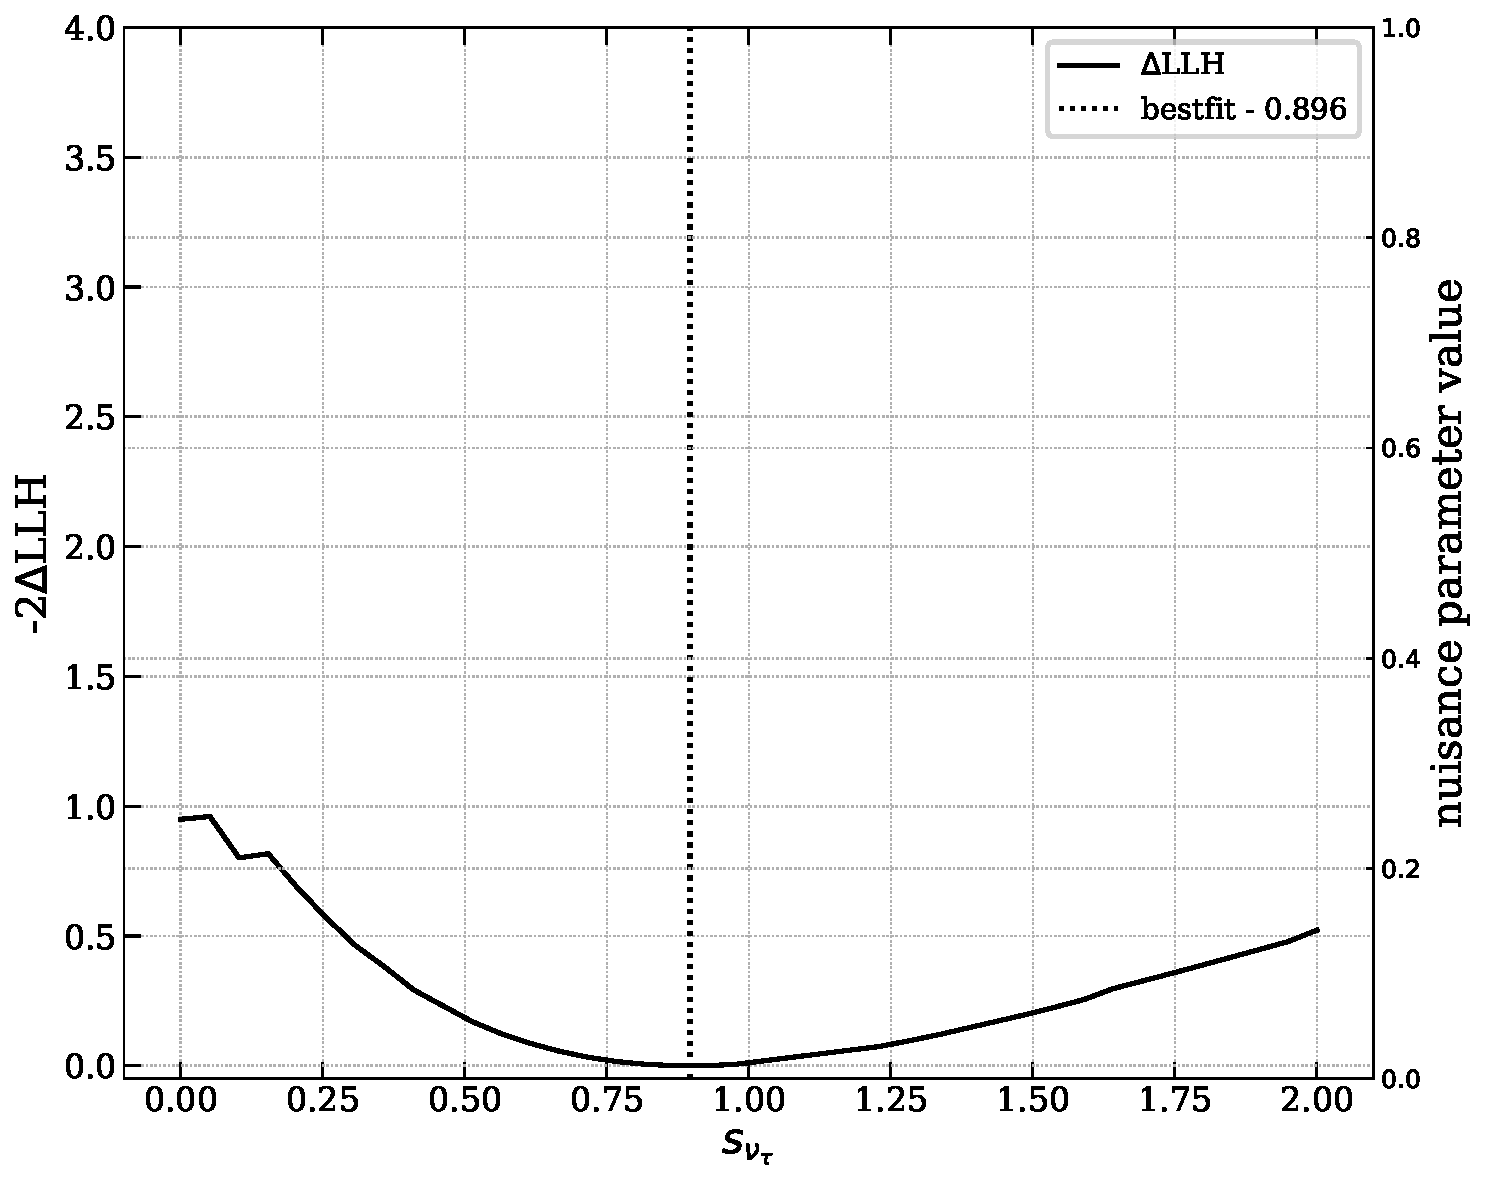
\includegraphics{./figures/results/profile_scan_astro_nutau_ratio.pdf}
    \end{subfigure}
    
    \caption[one dimensional profile likelihood scans of flavour scale factors $s_{\nu_{e}}$ and $s_{\nu_{\tau}}$]{1 dimensional profile likelihood scan of flavour scale factors $s_{\nu_{e}}$ (left) and $s_{\nu_{\tau}}$ (right). Solid black line corresponds to the profile likelihood, defined by the likelihood ratio $-2\Delta\mathrm{log}\mathcal{L}$ comparing a fixed value to the best fit value (denoted by dotted line).}
    \labfig{1d_llh}
\end{figure*}

\begin{figure}[h!]
    
    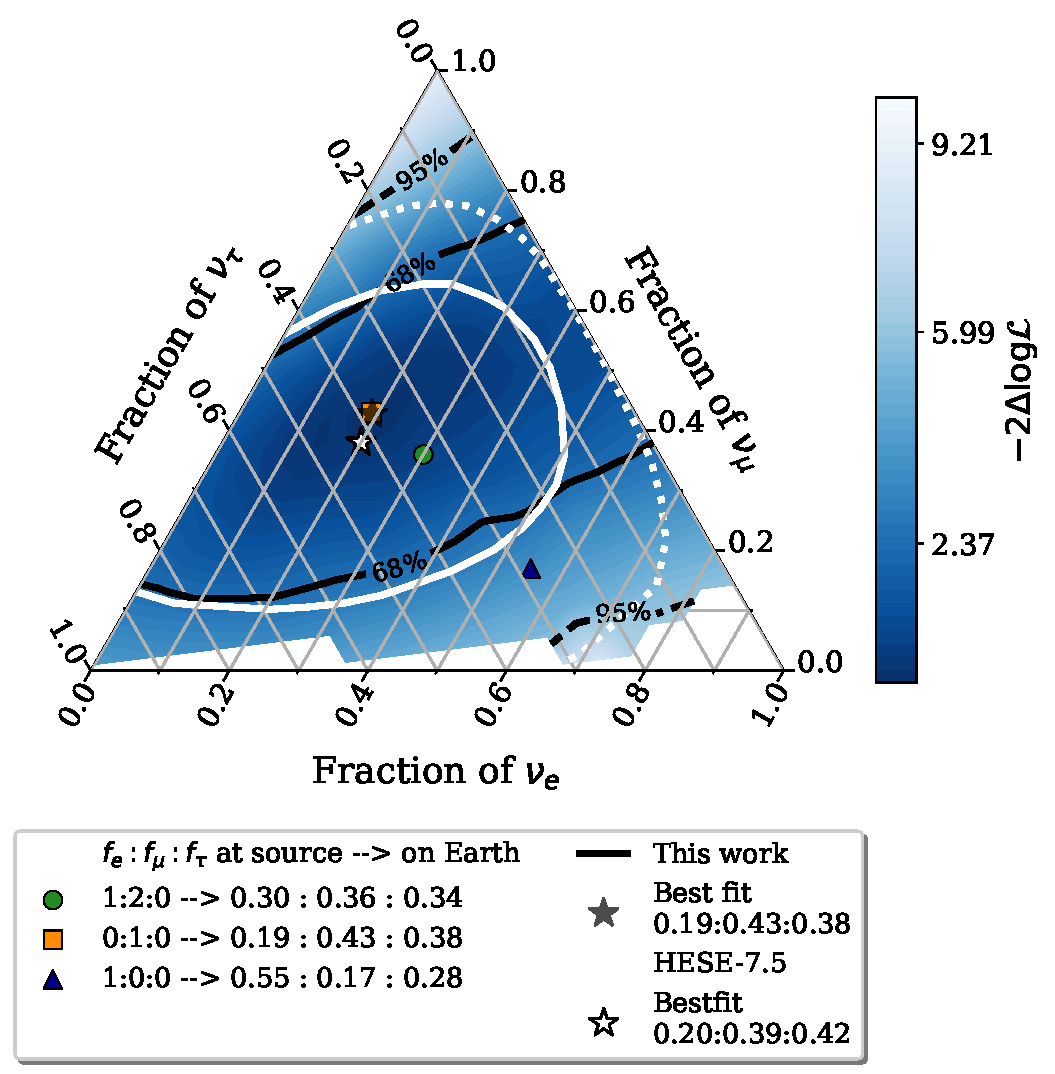
\includegraphics{./figures/results/HESE12_fancy_coverage_say_withhese7.pdf}
    \caption[Profile likelihood scan of the astrophysical neutrino flavor composition at Earth]{A 2 dimensional profile likelihood scan of the astrophysical neutrino flavour composition at Earth using 12 years of HESE data, classified in three event morphologies (see text for details). Each point on the triangle corresponds to a flavour composition of $f_{\nu_e}:f_{\nu_{\mu}}:f_{\nu_{\tau}}$ which can be read off the axes along the tick directions specified. The best fit flavour composition of 0.19 : 0.43 : 0.38 is indicated with a white star. The white solid and dashed lines represent the 68\% and 95\% confidence regions, respectively, obtained from the $\chi^2$-approximation using Wilk's theorem. Three flavour compositions expected at Earth from different source scenarios are also marked (\ref{sec:cosmic_nu}). The best fit flavour composition of a previous measurement that used 7.5 years of HESE data is indicated in grey star, with the 68\% and 95\% confidence regions represented by the grey solid and dotted lines, respectively \cite{Juliana_paper}.}

    \labfig{flavour_comp}
\end{figure}

\subsubsection{Why are the limits worse than the previous measurements?}
The best fit flavour composition $f_{\nu_e}:f_{\nu_{\mu}}:f_{\nu_{\tau}} = 0.19:0.43:0.38$ aligns well with the previous measurement \sidecite{Juliana_paper} of $f_{\nu_e}:f_{\nu_{\mu}}:f_{\nu_{\tau}} = 0.20:0.39:0.42$ (grey lines in \reffig{flavour_comp}). However, with 4 more years of data, which includes more double cascade events, it raises the question of why uncertainties are not shrinking. The reason is quite simple, the grey contours are derived using an extended likelihood, based on density estimates by producing a large number ($\sim10^6$ events per particle) of resimulations of 2 classified double cascades to assess the \textbf{tauness}. A dedicated algorithm (\texttt{RODEO}) was developed and used to compute the density estimate for sparse datasets produced from these resimulations in multiple dimensions (see \sidecite[-3cm]{Juliana_thesis} for details). Because of this, the limits one should actually compare with the previous measurement should be the one derived using \emph{the non-extended likelihood}, which is the same likelihood and PDF setup used for this iteration of the analysis.

\marginnote{\begin{kaobox}[title=\textbf{\emph{tauness}}]
    "Tauness" refers to the Bayesian posterior probability that an event is derived from a $\nu_{\tau}$ interaction. This can be approximated by analyzing the fraction of events in close proximity to the reconstructed properties of the data events, which are anticipated to result from $\nu_{\tau}$ interactions. In essence, tauness provides insight into the probability of each double cascade originating from a $\nu_{\tau}$ interaction compared to any other type of interaction.
\end{kaobox}}

\reffig{HESEall68} shows such a comparison. The best fit flavour composition $f_{\nu_e}:f_{\nu_{\mu}}:f_{\nu_{\tau}} = 0.19:0.43:0.38$ measured using this analysis (black lines) aligns well with the previous measurement of $f_{\nu_e}:f_{\nu_{\mu}}:f_{\nu_{\tau}} = 0.29:0.43:0.28$ (blue lines) using the same likelihood. Although not significantly, the limits derived from this iteration do get better along the $\nu_{\mu}$ fraction. Only 68\% CL contours  are shown.

\begin{figure}[h!]
    \caption[Profile likelihood scan of the astrophysical neutrino flavor composition at Earth, comparison with HESE-7.5 non extended likelihood]{The best fit flavour composition of 0.19 : 0.43 : 0.38 (black), using 12 years of HESE data (this work) compared with the best fit flavour composition of a previous measurement that used 7.5 years of HESE data \cite{Juliana_paper}. Comparison is shown by using the same likelihood formulation. The solid and dashed lines represent the 68\% and 95\% confidence regions, respectively, obtained from the $\chi^2$-approximation using Wilk's theorem. Three flavour compositions expected at Earth from different source scenarios (explained in Section~\ref{sec:flavor_theory}) are also marked.}
    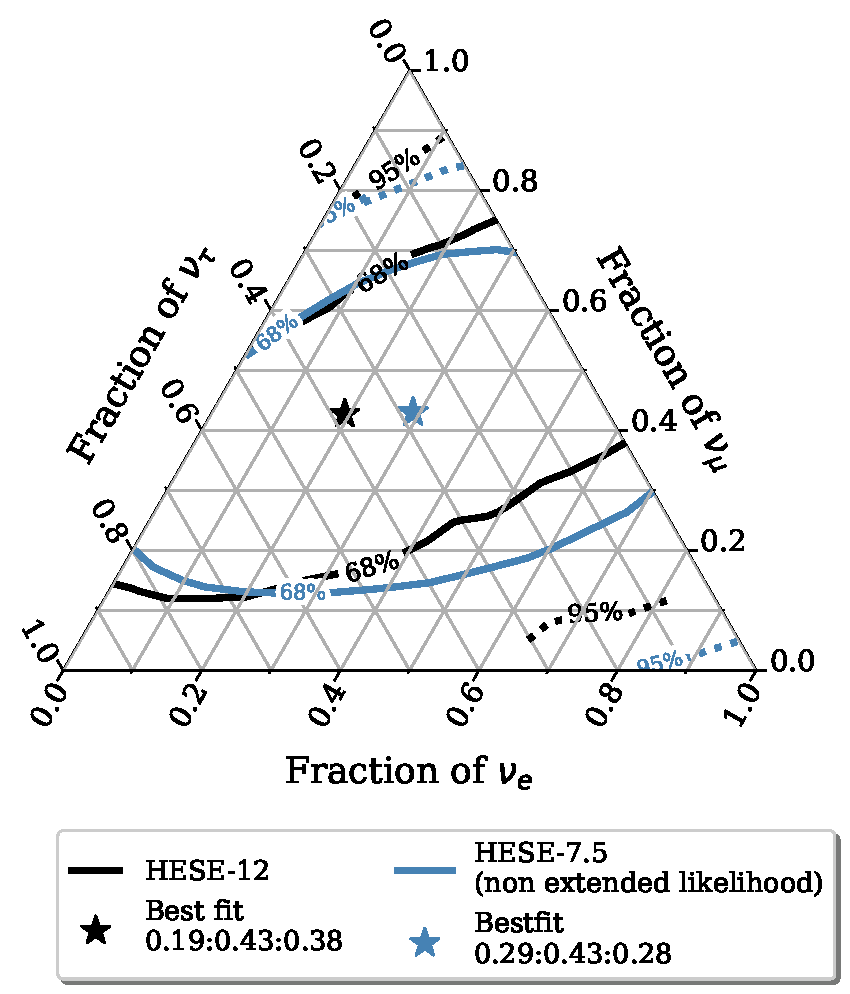
\includegraphics{./figures/results/HESE7and12_nonextendedonly.pdf}


    
    \labfig{HESEall68}
\end{figure}


\subsubsection{Comparison of sensitivities and derived constraints}
\label{sec:sens_bf}
The setup and all the relevant updates to the sample and selection chain for the analysis presented in this thesis were done using the best fit values from the previous analysis. The two signal parameters that affect the flavour measurement, especially the $\nu_{\tau}$ fraction and hence the double cascade events, are the index of the primary neutrino energy spectrum $\gamma_{\mathrm{astro}}$ (assuming a single power law) and the normalization. A harder spectrum (low $\gamma_{\mathrm{astro}}$) leads to a larger fraction of  high-energy events , while a softer spectrum (high $\gamma_{\mathrm{astro}}$) leads to a lower fraction of high-energy flux for samples with a similar effective area. This point was discussed in section \ref{sec:sensitivty} while discussing the sensitivity of the analysis. The analysis setup and sensitivity were shown using a spectrum with an index of 2.87, which is almost identical to the best fit value for this analysis (2.84) assuming equal partition of the neutrino flavour ($f_{\nu_e}:f_{\nu_{\mu}}:f_{\nu_{\tau}} = 0.33 : 0.33 : 0.33$). The estimated sensitivity projected much tighter constraints on 2D flavour measurements, specifically along the $\nu_{\tau}$ axis (see \reffig{sensitivity}). To understand the lack of improvement to reduce degeneracy along the $\nu_{e}$/$\nu_{\tau}$ axis, the sensitivity of the flavour measurement was recalculated using the best fit parameters from this analysis.

\begin{figure}
    
    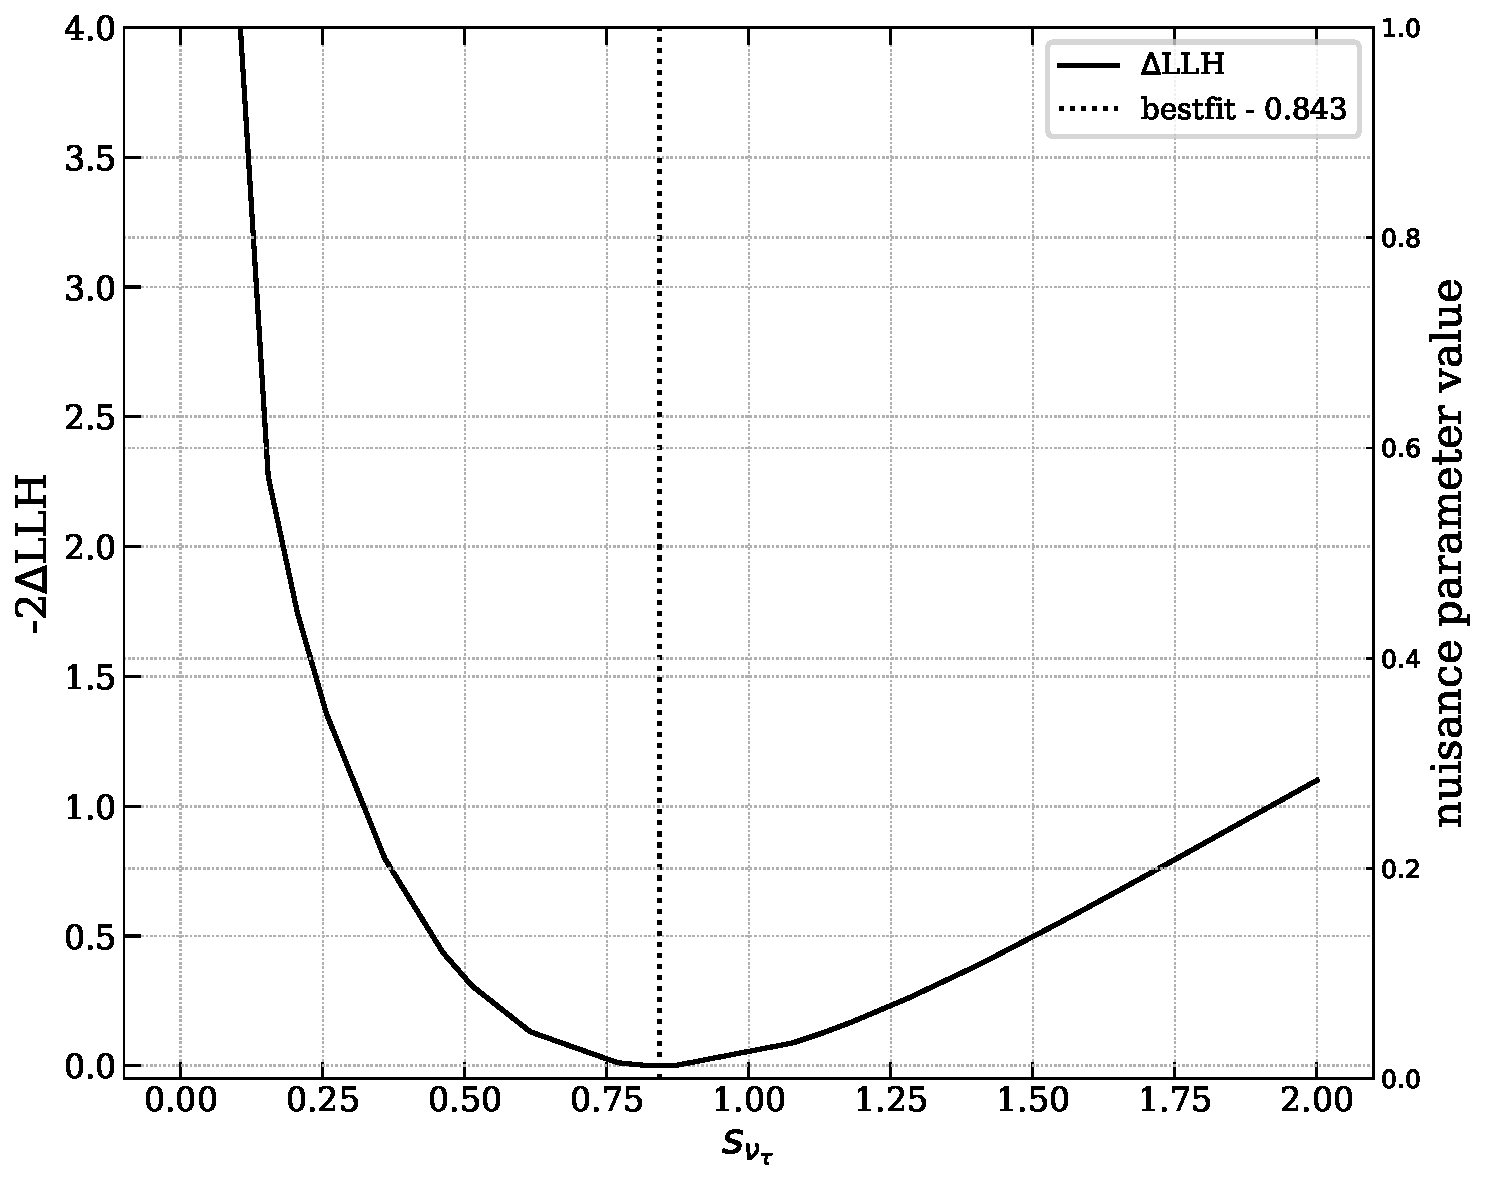
\includegraphics{./figures/results/simulation_profile_scan_astro_nutau_ratio.pdf}
    
    \caption[1D profile likelihood scan of $s_{\nu_{\tau}}$ using simulation]{1 dimensional profile likelihood asimov scan of $\nu_{\tau}$ scale factor, $s_{\nu_{\tau}}$ using \textbf{simulation} injected at best fit point. Solid black line corresponds to the profile likelihood, defined by the likelihood ratio $-2\Delta\mathrm{log}\mathcal{L}$ comparing a fixed value to the best fit value (denoted by dotted line).}
    \labfig{profile_llh_nutau_sim}

\end{figure}

The expected flavour constraints at 68\% CL is shown (maroon lines) in \reffig{PEs}. It is determined by using an asimov dataset \sidecite{asimov} created with the best fit values of all signal and nuisance parameters from \reftab{bf_signal} and \reftab{bf_nuisance}. For the sake of simplicity in comparison, a Poisson likelihood was utilized, as SAY likelihood tends to yield more conservative limits by construction (see Section~\ref{sec:SAY}). Constructing pseudotrials where data is drawn from SAY likelihood is not straightforward, therefore, to maintain consistency in comparisons, all fits depicted in \reffig{PEs} are computed using Poisson Likelihood. Consequently, the 68\% data limits displayed on the same plot (black line) are narrower compared to those shown in \reffig{flavour_comp}. Additionally, there is a slight shift in the best fit point. The key point here is that, given these signal parameters, the analysis is sensitive not only to measure a non-zero $\nu_{\tau}$ fraction, but also to reject it with better significance (approximately $3\sigma$ as shown in \reffig{profile_llh_nutau_sim} - the 1D profile likelihood scan of $s_{\nu_{\tau}}$ for the asimov dataset used to derive the 2D limits shown in \reffig{PEs}). The sensitivity results give rise to three questions, that will be discussed

\textbf{Are the constraints derived from data reliable?}\\
The contours shown in \reffig{flavour_comp} are based on the assumption that Wilk's theorem holds. This theorem states that the $-2\Delta\mathrm{log}\mathcal{L}$ approximately follows a $\chi^2$-distribution with $k = \text{dof}(\hat{\theta}, \hat{\xi}) - \text{dof}(\theta_t, \xi_t)$, where $\text{dof}(\theta, \xi)$ represents the number of free parameters in the fit. In the case of the flavour fit, there are 2 free parameters - $s_{\nu_{e}}$ and $s_{\nu_{\tau}}$. It is important to note that Wilk's theorem is only valid if the sample size is large and the model parameters are not bounded. However, the HESE sample is relatively small with only a few events passing all selection cuts. Additionally, the available Monte Carlo statistics are not large enough to provide sufficient statistics in every bin of the analysis histograms. Furthermore, the parameters are bounded as the flavour fractions cannot be negative. Therefore, it is essential to verify the validity of Wilk's theorem given these conditions. 

The validity of Wilk's theorem was tested for a few points on the 68\% and 95\% contours. This was achieved by generating pseudo datasets, each injected with a specific flavour composition (a point on the contour), while keeping the rest of the fit parameters at their best fit values, details of which can be found in Appendix~\ref{ch:wilks}. Each trials are fitted twice, once with a special case of flavour fractions (the one dataset was injected with), and again by leaving all the parameters free. A likelihood ratio is constructed for each trials by taking ratio of likelihood of \emph{the conditional fit} (fixed flavour fractions) to \emph{the free fit}. The distribution of the constructed likelihood ratio (Test Statsic) is compared with a $\chi^2$ distribution with 2 degree of freedom\sidenote{degree of freedom is 2 as both of the signal parameters are fixed simultaneously}. The results agrees well with $\chi_{k=2}^2$ with minor deviations that can be explained by the fact that the two parameters of interest are correlated and hence the degree of freedom is expected to be lower than 2.  
     
\textbf{Is deriving sensitivity using an asimov dataset a good choice?}\\
The Asimov dataset is a convenient alternative to generating a large number of pseudo trials for testing a specific realization. Computing the test statistic distribution of both conditional and global best fit values for each point in the triangle is quite expensive. It should not be assumed that the test statistic value that maximizes the likelihood of the Asimov dataset is always equal to the median of the test statistics derived from the full distribution of various pseudo experiments. 

To test this, sensitivity was derived using Monte Carlo pseudotrials, similar to the one described before for wilks' validity, but this time the fixed point for all trials was kept at the data best fit point, see Appendix~\ref{ch:sensitivity_checks} for details. In \reffig{PEs}, each point denoted with a marker "+" represents the points for which pseudo datasets were generated. Each dataset was generated by injecting the point denoted with "+" and fitted twice: once by keeping $s_{\nu_{e}}$ and $s_{\nu_{\tau}}$ fixed at the data best fit values (from \reftab{bf_signal}) and once with them free. This was done to test if the true flavour fraction is what the data fit returns and with what confidence the injected point can be rejected. The result is shown in Figure \reffig{PEs}. The color scheme shows the confidence level each point has to reject the null hypothesis (data best fit in this case). As can be seen, the pseudo-trial distribution matches quite well with the Asimov sensitivity. In fact, it predicts even tighter constraints compared to the Asimov case.

\begin{figure}[h]
    
    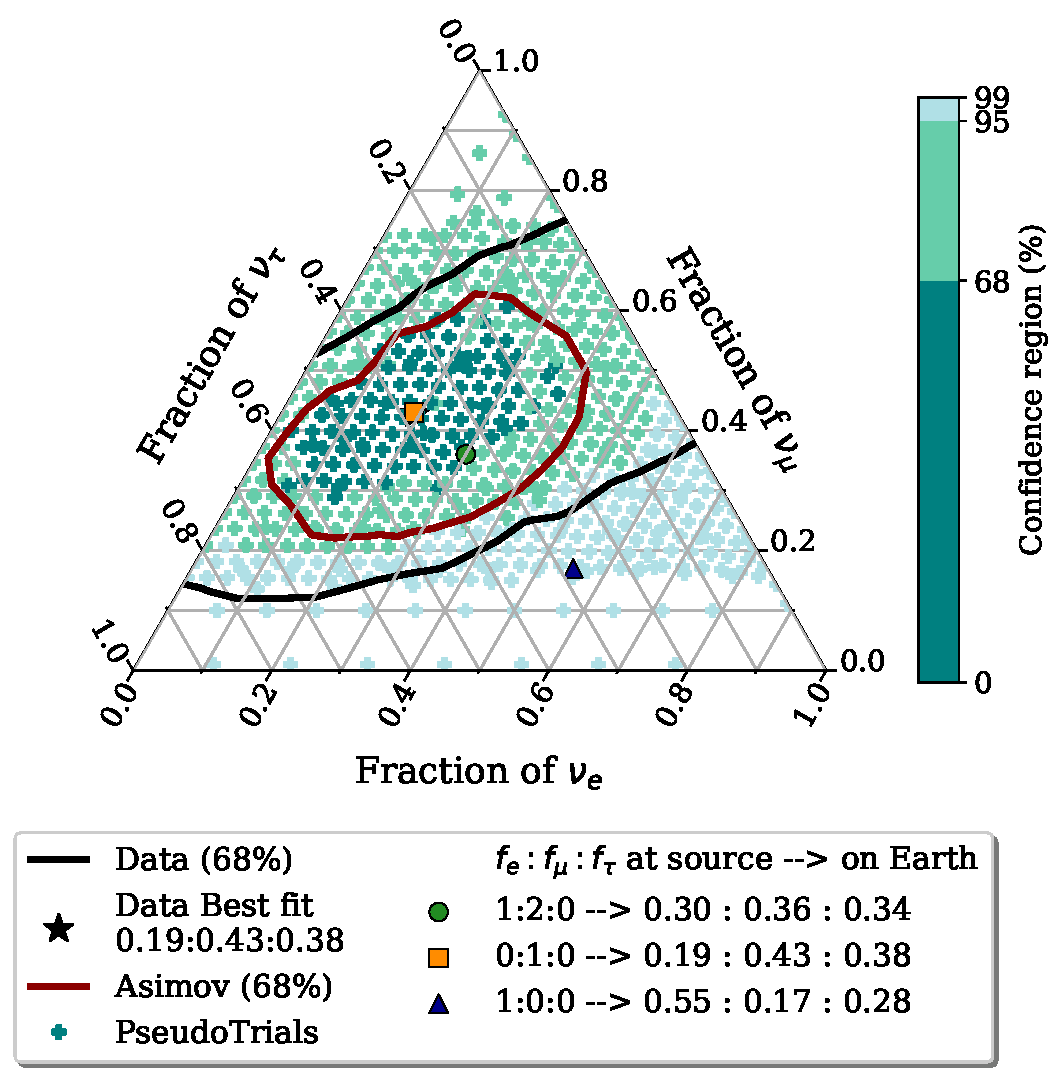
\includegraphics{./figures/results/PE_data_asimov_68.pdf}


    \caption[Comparison of Measured flavoured ratio with asimov sensitivity and pseudo trials]{Comparison of Measured flavoured ratio (black line) with asimov sensitivity(maroon line) and pseudo trials (marked with '+'). Each + represents a pseudo dataset, drawn from flavour composition of that very point. Colorbar shows confidence intervals of each of these points, to reject the best fit flavour composition of $f_{\nu_e}:f_{\nu_{\mu}}:f_{\nu_{\tau}} = 0.19:0.43:0.38$. All other parameters of the fit are injected at their best fit values.}
    \labfig{PEs}
\end{figure}

\textbf{Are the double cascades found in the data a unusual realization of the expectations?}\\

Forward-folding fits, as described in section \ref{sec:analysis}, heavily relies on the expected values for each bin of the analysis histograms. It is crucial to choose reliable variables so that the likelihood space looks different for signal and background. For this reason, the analysis variables for double cascade bins are different from those for cascades and tracks. This is because the zenith distribution of astrophysical $\nu_{\tau}$ flux shows no significant variation between signal and background. The PDF used in this case was selected due to the correlation of the Tau decay length ($\mathrm{L}_{\mathrm{dc}}$) with the energy of the second cascade ($\mathrm{E}_{2}$) for double cascades resulting from $\nu_{\tau}$-cc interactions, contributing to the population of signal events along this diagonal (see \reffig{LvsE_signalbkg}), while the background lacks this correlation. The 2D Monte Carlo PDF at best fit, shown in \reffig{LvsE_datamc}, shows the  Monte Carlo events populating the bins along the diagonal. However, the data events are in regions where the background population is expected background density is equally high. While drawing data using poisson distribution, fluctuations around the best fit are considered which in principle should give all possible realisations of the data events ending up in bins with high expectations. Only a small subset of pseudo-datasets generated with this PDF will produce events that are similar to the observed data. Therefore, in addition to the previously described pseudotrials, only the trials with histograms that included events in regions predominantly occupied by background-like events were retained for the sensitivity study. This approach helps verify whether the limits derived from this subset of trials resemble those obtained from the actual data.
\begin{figure}[h!]
    
    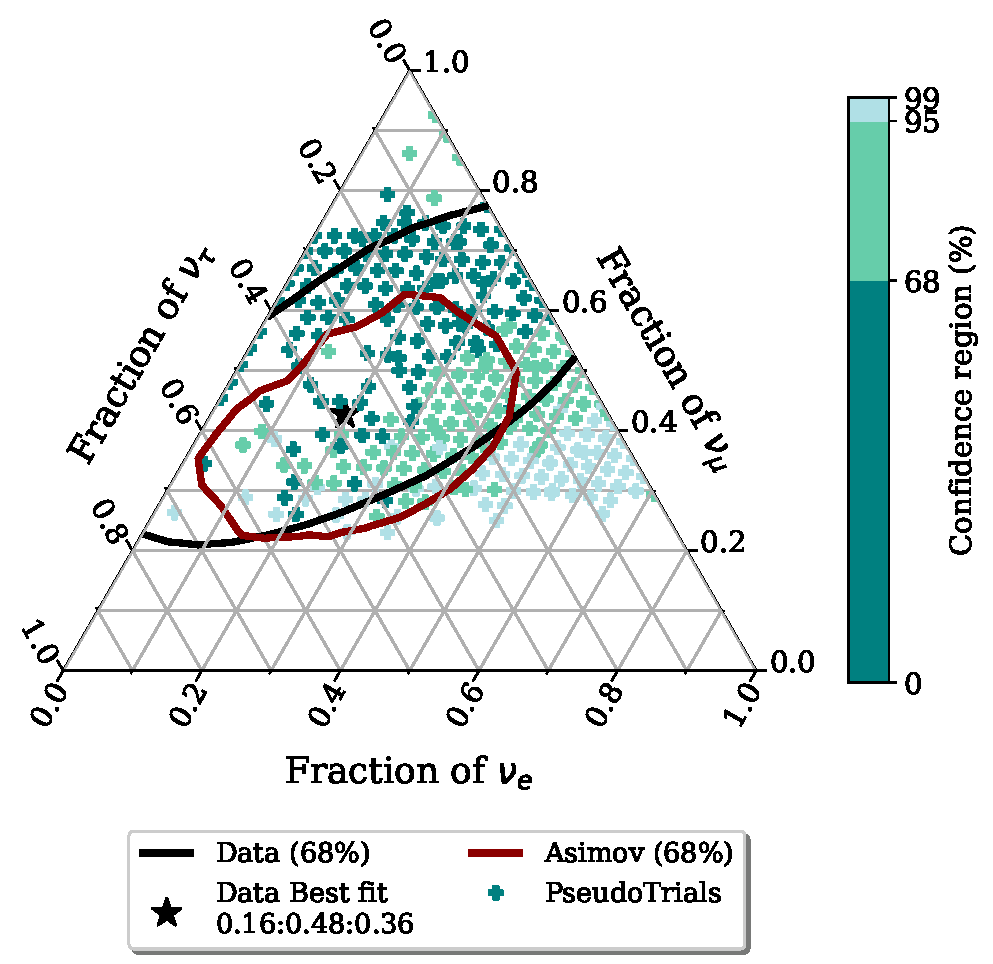
\includegraphics{./figures/results/PE_data_asimov_68_BkgOnly.pdf}


    \caption[Comparison of Measured flavoured ratio with asimov sensitivity and pseudo trials, with subset of trials having low signal/background analysis PDFs]{Comparison of Measured flavoured ratio (black line) with asimov sensitivity(maroon line) and pseudo trials (marked with '+'). Each + represents a pseudo dataset, drawn from flavour composition of that very point. Colorbar shows confidence intervals of each of these points, to reject the best fit flavour composition of $f_{\nu_e}:f_{\nu_{\mu}}:f_{\nu_{\tau}} = 0.19:0.43:0.38$. Only trials with final histogram in three lower energy bins are kept in TS distribution. All other parameters of the fit are injected at their best fit values.}
    \labfig{PEs_bkg}
\end{figure}
Ideally, one would generate pseudo trials until all the Poisson-distributed events fall within the same region of the PDF as shown in \reffig{LvsE_datamc}. However, this approach was found to be computationally expensive. For instance, each dataset displayed (around 500) in \reffig{PEs} was produced from 500 trials, with each trial fitted twice. On average, each fit took approximately one hour to complete. Therefore, before proceeding, the proportion of PDFs that did not meet the cut criteria was estimated to determine whether using computational resources for further trials was justified. Several tested datasets from different regions of the triangle revealed that, for most datasets, only about 20\% of the 500 trials resulted in final histograms with events concentrated in the lower energy bins. There was no feasible way to generate a sufficient number of trials to reduce statistical errors and set definitive limits. As a workaround, only the small proportion of trials that met the necessary criteria were used to generate the TS distributions, allowing an update of the sensitivity shown in \reffig{PEs}. This updated result is presented in \reffig{PEs_bkg}. As evident from the vanished points, not only were most of the trials excluded, but the confidence intervals also became significantly larger—especially along the $\nu_{\tau}$ axis—aligning more closely with the data limits. This concludes why both asimov sensitivity and pseudo trials in \reffig{PEs} showed such tight constraints. 



\section{Discussion}
\label{sec:results_discussion}

The analysis setup and particle identification methods developed and refined throughout this thesis demonstrate that IceCube has sufficient sensitivity to measure the flavour ratios of the astrophysical neutrino spectrum and impose stringent constraints. However, further refinement of techniques, particularly for reconstructing double-cascade events, is necessary. With additional years of data, not only do we gain more neutrino events, but our understanding of the detector’s performance also deepens. Consequently, reconstruction techniques should be re-evaluated using newer, updated simulations to better represent a realistic sample of events. Although this analysis did not yield statistically significant results, it identified several issues that raise concerns about the purity of the double-cascade sample. For instance, changing the ice model from SPICE-3.2.1 to SPICE-Bfr resulted in an increased number of classified double-cascade events, with some events being reclassified. Additionally, further investigation is needed into the false mean SPE template issue, which was identified but not fully explored. Since \texttt{millipede} reconstruction relies on these templates, excluding certain information may limit the detector’s effectiveness. These issues should be addressed thoroughly before making any further measurements with this classifier. Regarding the measured flavour ratio, as illustrated in \reffig{flavour_comp}, the best fit suggests sources dominated by a muon-damped production scenario; however, with the derived uncertainties, no production scenario is significantly preferred. The neutron beam scenario (source ratio $f_{\nu_e}:f_{\nu_{\mu}}:f_{\nu_{\tau}} = 1:0:0$, evolving to 0.55:0.17:0.28 on Earth) is disfavored by roughly $1\sigma$ but remains consistent within $2\sigma$.

A specific measurement of the neutrino energy spectrum was not part of the analysis presented here, as the focus was primarily on flavour measurement, with efforts directed toward improving particle identification. Nonetheless, the HESE sample could also be used to measure, and potentially search for, spectral features. Recent independent studies have discovered a spectral break in the neutrino spectrum at around 30 TeV, softening the spectrum at higher energies, which is within the range of this analysis \sidecite{globalfit_icrc,MESE_icrc}. This finding offers insight into why previous measurements targeting different energy ranges produced significantly different spectral indices for a single power-law spectrum \sidecite{HESE7_sample,diffusenumu,cscd_6yr}. Since the HESE sample focuses on high-energy events, where no such spectral features have been observed, and has much lower statistical power than those other samples, no spectral feature searches were attempted during this work.

A less model-dependent approach to describing the astrophysical neutrino flux is the differential unfolding of the energy spectrum. This method divides the flux into energy bins, where each bin is fit independently with a constant $\sim\mathrm{E}^{-2}$ spectrum, rather than assuming a continuous power-law across the entire energy range. Ideally, this unfolding would be performed separately for each neutrino flavour to avoid assuming a uniform spectral shape for all flavours. Measuring the flavour composition as a function of energy would also be valuable, as neutrino production processes are energy-dependent. However, due to the limited statistical power of the current dataset, meaningful results could not yet be obtained.

Finally, improvements in reconstruction methods and more data are necessary for future experiments to shed more light on flavour measurements. Double-cascade reconstruction currently has an upper energy limit, as higher-energy events are only partially contained within the detector due to their geometry. In addition, improved detection hardware could provide better information on photon charge and direction, enhancing the overall reconstruction process. These points, along with the potential to constrain the flavour composititons of astrophysical neutrinos for a proposed new generation of neutrino detectors, will be discussed in detail in the next chapter. 


